\documentclass{article}
\usepackage[T1]{fontenc}
\usepackage{lmodern}
\usepackage{graphicx}
\usepackage{amsmath,amssymb}
\usepackage[a4paper,margin=2cm]{geometry}
\usepackage[absolute,overlay]{textpos}
\setlength{\TPHorizModule}{1mm}
\setlength{\TPVertModule}{1mm}
\usepackage[indonesian]{babel}
\usepackage{hyperref}
\setlength{\emergencystretch}{2em}
\title{09-Beberapa-block-cipher-bagian1-2026}
\author{pdf\_ppt\_to\_latex}
\date{}

\begin{document}

% --- unit llm 1 ---
% === Halaman 1 (llm) ===

\begin{center}
Bahan kuliah IF4020 Kriptografi

{\huge \textcolor{red}{09- Review Beberapa Block Cipher}}

{\Large \textcolor{red}{(Bagian 1: DES dan Triple DES)}}

\vspace{20mm}

Oleh: Rinaldi M

\vspace{10mm}

Program Studi Teknik Informatika\\
Sekolah Teknik Elektro dan Informatika\\
Institut Teknologi Bandung\\
2026
\end{center}

\newpage

% --- unit llm 2 ---
% === Halaman 2 (llm) ===

\vspace{151.47mm}

Data Encryption Standard (DES)

% deskripsi: Teks dekoratif berwarna biru 'DES Data Encryption Standard'
% bbox normalisasi: [0.0300, 0.2700, 0.3200, 0.7800]
\begin{textblock*}{60.90mm}(6.30mm,80.19mm)
\noindent
\includegraphics[width=60.90mm,height=151.47mm]{images/llm/page_002_img_01.png}%
\end{textblock*}

\newpage

% --- unit llm 3 ---
% === Halaman 3 (llm) ===

\section*{Sejarah DES}

\begin{itemize}
    \item Pada tahun 1972 NIST meminta standard enkripsi \textit{cipher} blok.
    \item Pada tahun 1974 Horst Feistel di IBM mendesain cipher blok \textit{Lucifer} (panjang kunci 128 bit, Panjang blok 128 bit)
    \item \textit{Lucifer} kemudian berkembang menjadi DES dengan beberapa masukan dari NSA (\textit{National Security Agency}):
    \begin{itemize}
        \item panjang kunci 56 bit, ukuran blok 64 bit
        \item 16 putaran.
    \end{itemize}
    \item Tahun 1976 DES disetujui oleh \textit{National Bureau of Standard} (NBS) setelah penilaian kekuatannya oleh NSA.
    \item Sejak itu DES diimplementasikan secara luas, baik \textit{software} maupun \textit{hardware}.
\end{itemize}

\newpage

% --- unit llm 4 ---
% === Halaman 4 (llm) ===

\vspace{181.17mm}

\begin{itemize}
    \item Catat bahwa DES adalah sebah standard, sedangkan algoritmanya sendiri bernama DEA (\textit{Data Encryption Algorithm}). Kedua nama ini sering dikacaukan.
    \item DES termasuk ke dalam algoritma kriptografi kunci-simetri dan tergolong ke dalam \textit{cipher} blok.
    \item DES beroperasi pada ukuran blok plainteks 64 bit.
    \item Panjang kunci ekternal = 64 bit (sesuai ukuran blok), tetapi hanya 56 bit yang dipakai (8 bit \textit{parity} tidak digunakan). Bit parity = bit ke-8, 16, 24, dst.
\end{itemize}

% deskripsi: Gambar sampul dokumen FIPS PUB 46 berjudul 'DATA ENCRYPTION STANDARD'
% bbox normalisasi: [0.6800, 0.1600, 0.9400, 0.7700]
\begin{textblock*}{54.60mm}(142.80mm,47.52mm)
\noindent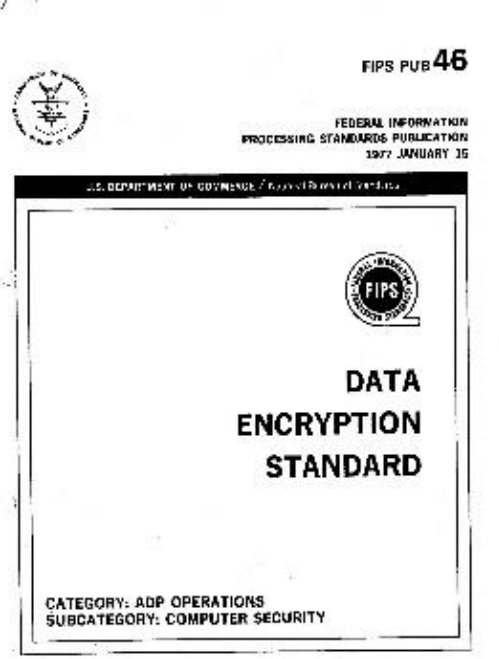
\includegraphics[width=54.60mm,height=181.17mm]{images/llm/page_004_img_01.png}%
\end{textblock*}

\newpage

% --- unit llm 5 ---
% === Halaman 5 (llm) ===

\begin{itemize}
    \item Setiap blok plainteks dienkripsi dalam 16 putaran \textit{enciphering}.
    \item Setiap putaran menggunakan kunci internal (kunci putaran) berbeda.
    \item Kunci internal sepanjang 48-bit dibangkitkan dari kunci eksternal
    \item Setiap blok plainteks mengalami permutasi awal (\textit{IP}), 16 putaran \textit{enciphering}, dan inversi permutasi awal (\textit{IP}^{-1}). (lihat Gambar 1)
\end{itemize}

\newpage

% --- unit llm 6 ---
% === Halaman 6 (llm) ===

\vspace{92.07mm}

\vspace{10mm}
\textbf{Gambar 1 Skema global algoritma DES}

% deskripsi: Diagram alir skema global algoritma DES yang menunjukkan proses dari blok plainteks melalui Initial Permutation (IP), proses Enciphering yang diulang 16 kali dengan sub-key $K_i$, hingga Final Permutation ($IP^{-1}$) menjadi blok cipherteks, serta proses Key expansion dari kunci $K$.
% bbox normalisasi: [0.2800, 0.5000, 0.8900, 0.8100]
\begin{textblock*}{128.10mm}(58.80mm,148.50mm)
\noindent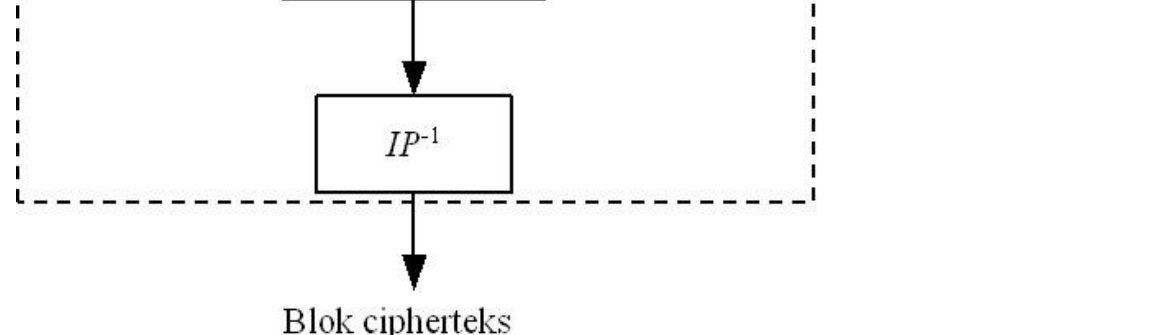
\includegraphics[width=128.10mm,height=92.07mm]{images/llm/page_006_img_01.png}%
\end{textblock*}

\newpage

% --- unit llm 7 ---
% === Halaman 7 (llm) ===

% (tidak ada teks dari model)

% deskripsi: Diagram alur proses enkripsi menggunakan jaringan Feistel 16-round, yang menunjukkan input plaintext P (64 bits), proses Initial Permutation (IP), ekspansi kunci K menjadi K1 sampai K16, proses Enciphering, Inverse Initial Permutation (IP-1), dan output ciphertext C (64 bits).
% bbox normalisasi: [0.0500, 0.0800, 0.9300, 0.8300]
\begin{textblock*}{184.80mm}(10.50mm,23.76mm)
\noindent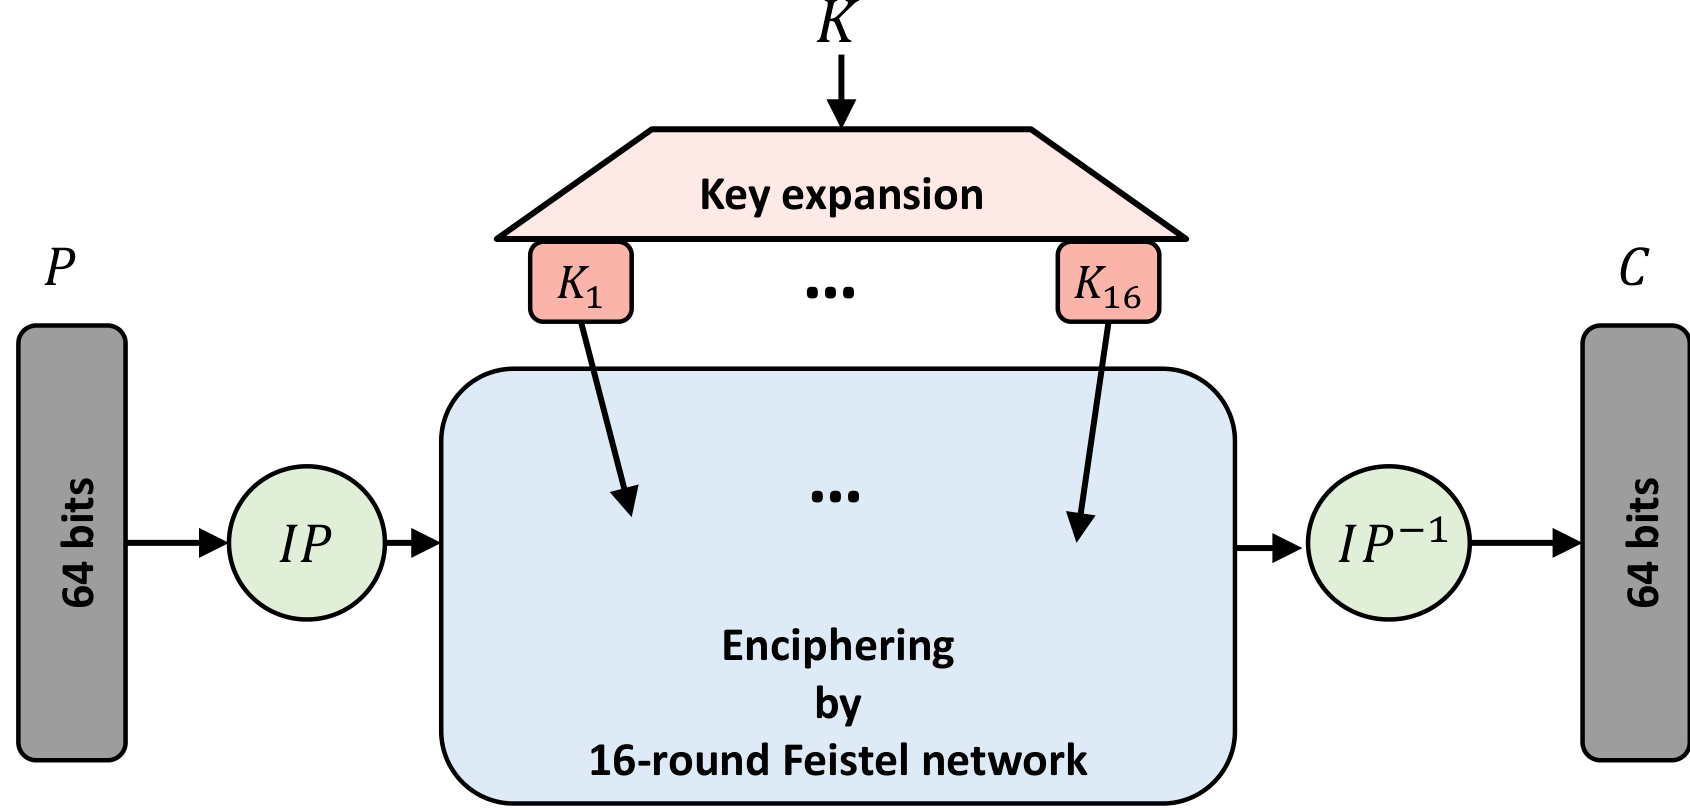
\includegraphics[width=184.80mm,height=222.75mm]{images/llm/page_007_img_01.png}%
\end{textblock*}

\newpage

% --- unit llm 8 ---
% === Halaman 8 (llm) ===

\vspace{158.00mm}

\vspace{50mm}
\begin{center}
\textbf{Gambar 2. Algoritma Enkripsi dengan DES}
\end{center}

% deskripsi: Diagram blok proses enkripsi DES yang terdiri dari dua bagian: ringkasan proses di sebelah kiri dan detail iterasi 16 round Feistel di sebelah kanan.
% bbox normalisasi: [0.0370, 0.4300, 0.9270, 0.9620]
\begin{textblock*}{186.90mm}(7.77mm,127.71mm)
\noindent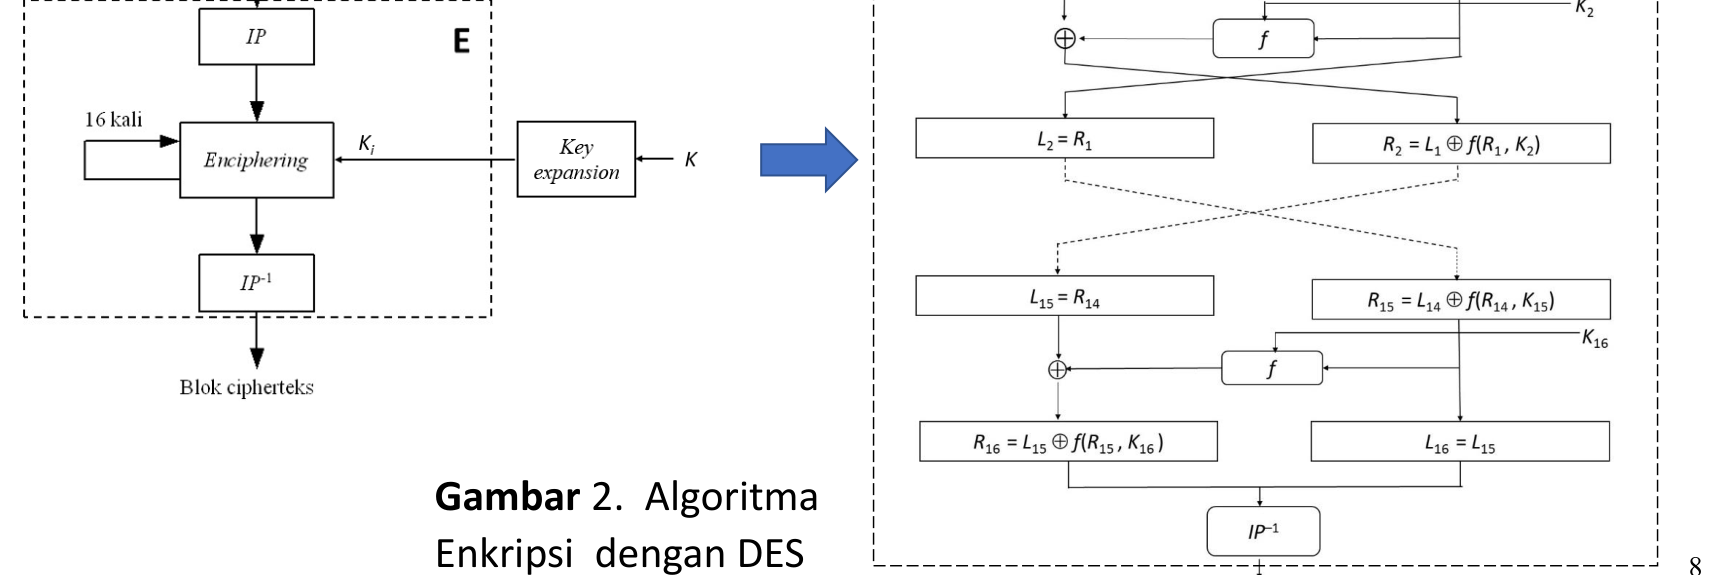
\includegraphics[width=186.90mm,height=158.00mm]{images/llm/page_008_img_01.png}%
\end{textblock*}

\newpage

% --- unit llm 9 ---
% === Halaman 9 (llm) ===

\vspace{178.20mm}

Sumber asli dari dokumen FIPS-PUB

% deskripsi: Diagram alir struktur algoritma enkripsi DES (Data Encryption Standard) yang menunjukkan proses permutasi awal, 16 ronde transformasi Feistel dengan kunci $K_1$ hingga $K_{16}$, dan permutasi akhir.
% bbox normalisasi: [0.3020, 0.3800, 0.6850, 0.9800]
\begin{textblock*}{80.43mm}(63.42mm,112.86mm)
\noindent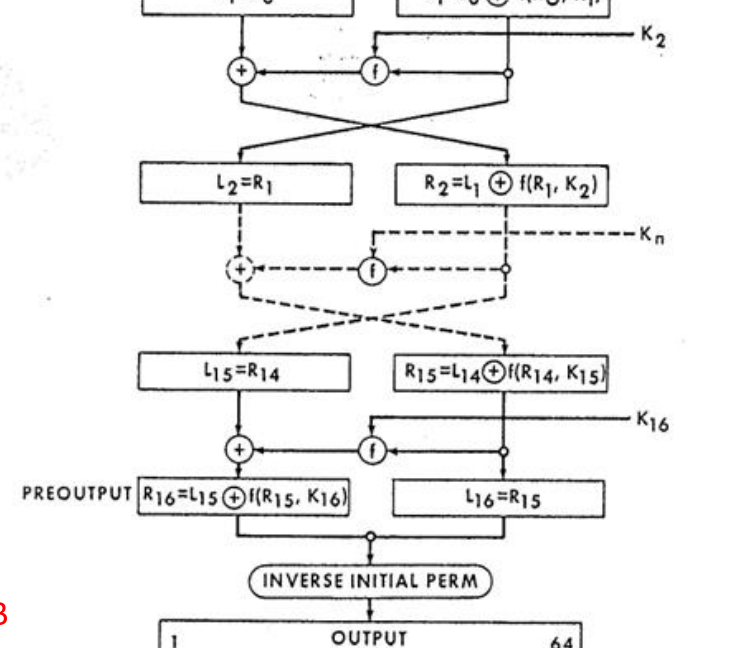
\includegraphics[width=80.43mm,height=178.20mm]{images/llm/page_009_img_01.png}%
\end{textblock*}

\newpage

% --- unit llm 10 ---
% === Halaman 10 (llm) ===

\section*{Pembangkitan Kunci Internal (\textit{key expansion})}

\begin{itemize}
    \item Kunci internal = kunci setiap putaran = \textit{subkey (round key)}
    \item Ada 16 putaran, jadi ada 16 kunci internal: $K_1, K_2, \dots, K_{16}$
    \item Kunci internal dibangkitkan dari kunci eksternal (64 bit) yang diberikan oleh pengguna. Di dalam dokumen resmi DES pembangkitan kunci internal disebut \textit{key schedule}.
    \item Panjang kunci internal adalah 48 bit
    \item Gambar 3 memperlihatkan proses pembangkitan kunci internal.
\end{itemize}

\newpage

% --- unit llm 11 ---
% === Halaman 11 (llm) ===

\vspace{10mm}

Gambar 3. Pembangkitan kunci internal

% deskripsi: Diagram alir proses pembangkitan kunci internal DES yang menunjukkan langkah-langkah dari Kunci eksternal 64 bit, melalui Permutasi PC-1, pembagian menjadi C dan D (masing-masing 28 bit), proses Left Shift berulang, hingga Permutasi PC-2 untuk menghasilkan kunci internal K1 sampai K16 dengan panjang 48 bit.
% bbox normalisasi: [0.0500, 0.1000, 0.6800, 0.9600]
\begin{textblock*}{132.30mm}(10.50mm,29.70mm)
\noindent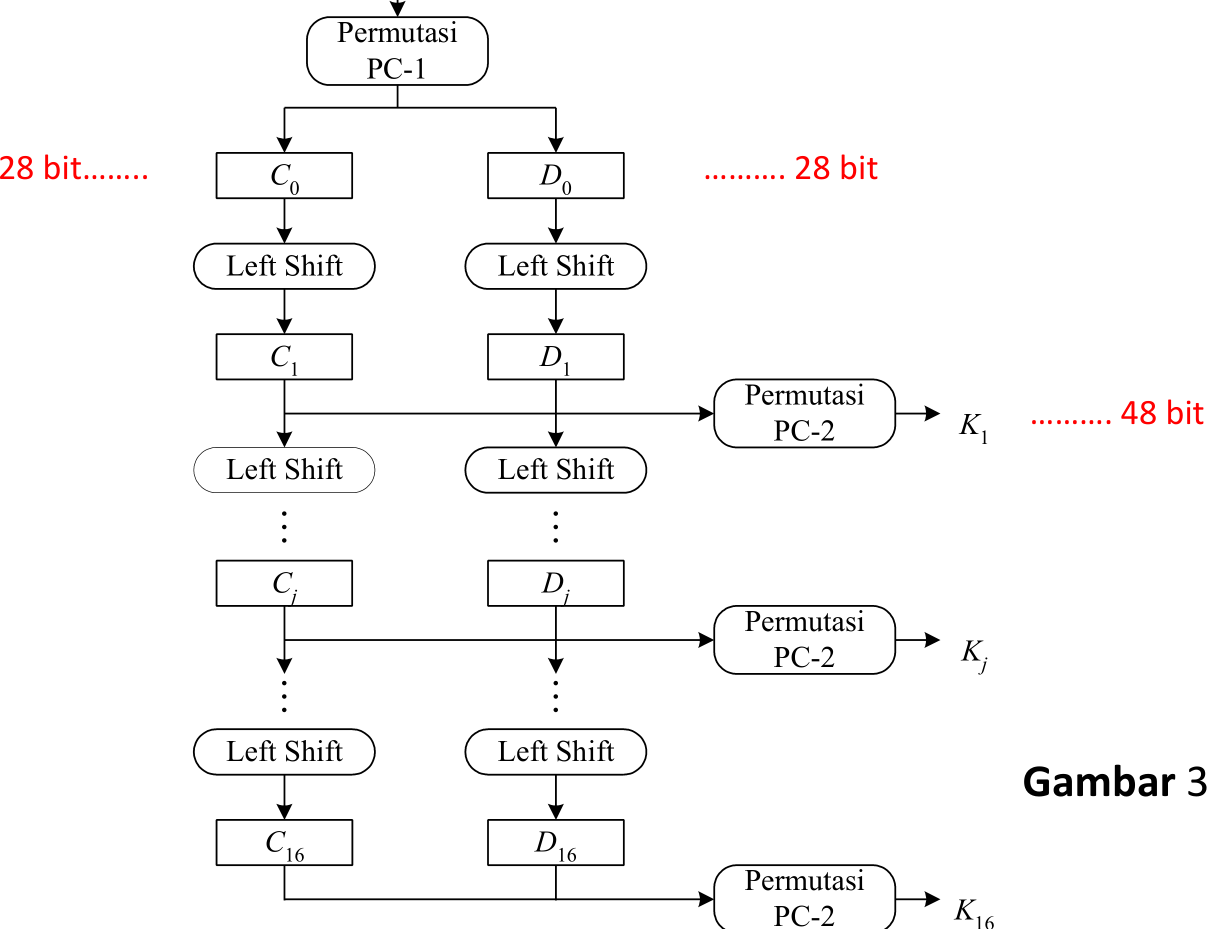
\includegraphics[width=132.30mm,height=255.42mm]{images/llm/page_011_img_01.png}%
\end{textblock*}

\newpage

% --- unit llm 12 ---
% === Halaman 12 (llm) ===

Sumber asli dari dari dokumen FIPS-PUB

\vspace{118.80mm}

% deskripsi: Diagram alir proses penjadwalan kunci (key scheduling) dalam algoritma enkripsi, yang menunjukkan transformasi kunci 64-bit melalui Permuted Choice 1, pemisahan menjadi dua bagian (C dan D), pergeseran kiri (left shift) berulang, dan penggunaan Permuted Choice 2 untuk menghasilkan kunci sub-kunci K1 hingga K16.
% bbox normalisasi: [0.3040, 0.5300, 0.6800, 0.9300]
\begin{textblock*}{78.96mm}(63.84mm,157.41mm)
\noindent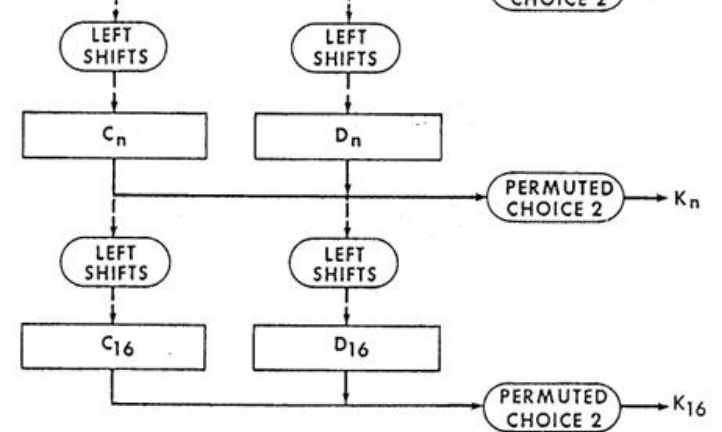
\includegraphics[width=78.96mm,height=118.80mm]{images/llm/page_012_img_01.png}%
\end{textblock*}

\newpage

% --- unit llm 13 ---
% === Halaman 13 (llm) ===

Matriks permutasi kompresi PC-1:

\vspace{10mm}

\textcolor{red}{Perhatikan, bit-bit parity, yaitu bit ke-8, 16, 28, ... dibuang, sehingga menjadi 56 bit}

\vspace{40mm}

$C_0$: berisi bit-bit dari $K$ pada posisi

\[
\begin{aligned}
&57, 49, 41, 33, 25, 17, 9, 1, 58, 50, 42, 34, 26, 18 \\
&10, 2, 59, 51, 43, 35, 27, 19, 11, 3, 60, 52, 44, 36
\end{aligned}
\]

$D_0$: berisi bit-bit dari $K$ pada posisi

\[
\begin{aligned}
&63, 55, 47, 39, 31, 23, 15, 7, 62, 54, 46, 38, 30, 22 \\
&14, 6, 61, 53, 45, 37, 29, 21, 13, 5, 28, 20, 12, 4
\end{aligned}
\]

% deskripsi: Tabel matriks permutasi kompresi PC-1 yang berisi angka-angka posisi bit.
% bbox normalisasi: [0.0600, 0.1080, 0.9400, 0.5020]
\begin{textblock*}{184.80mm}(12.60mm,32.08mm)
\noindent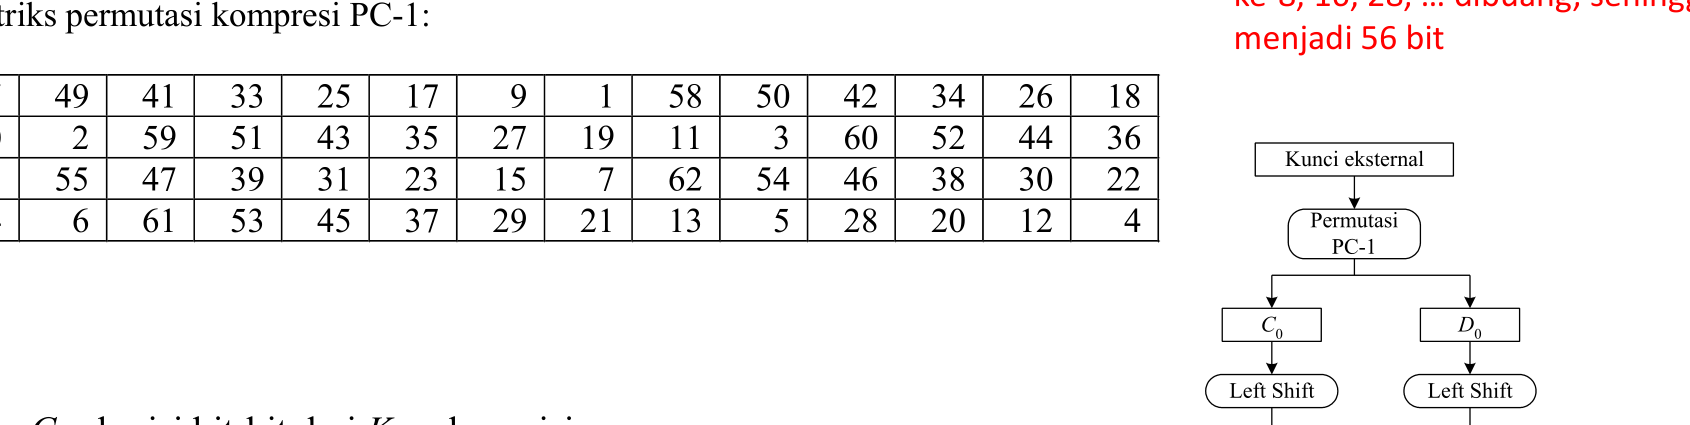
\includegraphics[width=184.80mm,height=117.02mm]{images/llm/page_013_img_01.png}%
\end{textblock*}

% deskripsi: Diagram alur proses penjadwalan kunci (key scheduling) DES, menunjukkan penggunaan Permutasi PC-1, Left Shift, dan Permutasi PC-2 untuk menghasilkan subkey K1 sampai K16.
% bbox normalisasi: [0.0600, 0.5180, 0.9400, 0.9120]
\begin{textblock*}{184.80mm}(12.60mm,153.85mm)
\noindent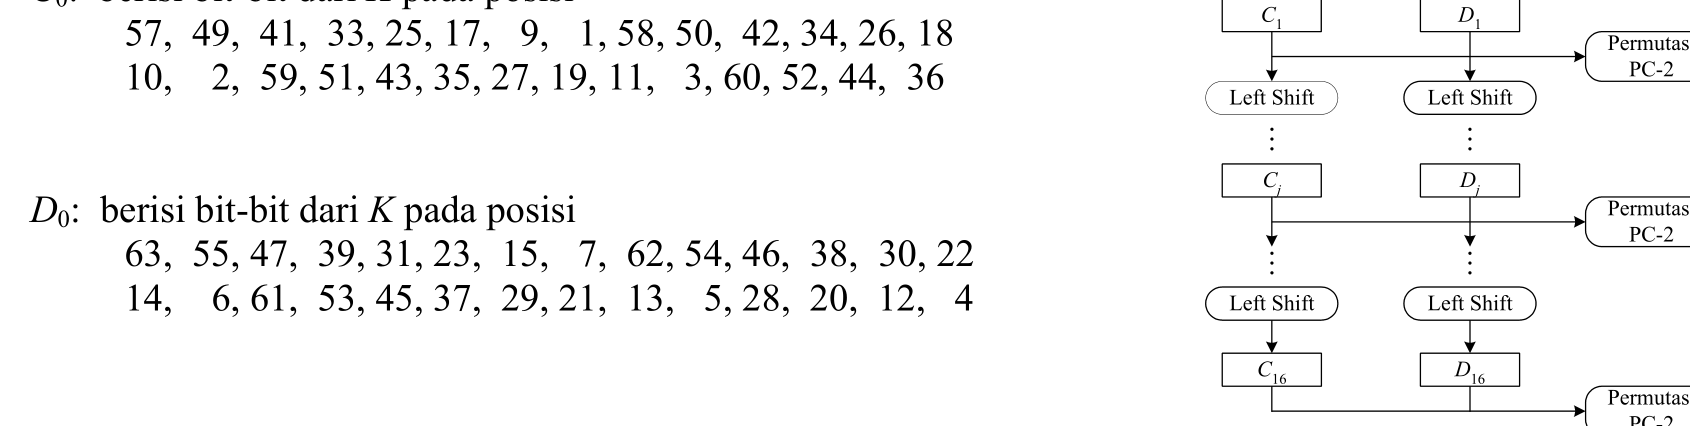
\includegraphics[width=184.80mm,height=117.02mm]{images/llm/page_013_img_02.png}%
\end{textblock*}

% bbox perkiraan otomatis: Tabel matriks permutasi kompresi PC-1 yang berisi angka-angka posisi bit.
% bbox perkiraan otomatis: Diagram alur proses penjadwalan kunci (key scheduling) DES, menunjukkan penggunaan Permutasi PC-1, Left Shift, dan Permutasi PC-2 untuk menghasilkan subkey K1 sampai K16.

\newpage

% --- unit llm 14 ---
% === Halaman 14 (llm) ===

\vspace{238.79mm}

\textbf{Tabel 1. Jumlah pergeseran bit pada setiap putaran}

\begin{tabular}{cc}
Putaran, $i$ & Jumlah pergeseran bit \\
\hline
1 & 1 \\
2 & 1 \\
3 & 2 \\
4 & 2 \\
5 & 2 \\
6 & 2 \\
7 & 2 \\
8 & 2 \\
9 & 1 \\
10 & 2 \\
11 & 2 \\
12 & 2 \\
13 & 2 \\
14 & 2 \\
15 & 2 \\
16 & 1 \\
\end{tabular}

% deskripsi: Diagram alir proses kriptografi yang menunjukkan langkah-langkah permutasi PC-1, pemisahan menjadi C dan D, operasi Left Shift berulang, dan permutasi PC-2 untuk menghasilkan kunci K1 hingga K16.
% bbox normalisasi: [0.0600, 0.1080, 0.9400, 0.9120]
\begin{textblock*}{184.80mm}(12.60mm,32.08mm)
\noindent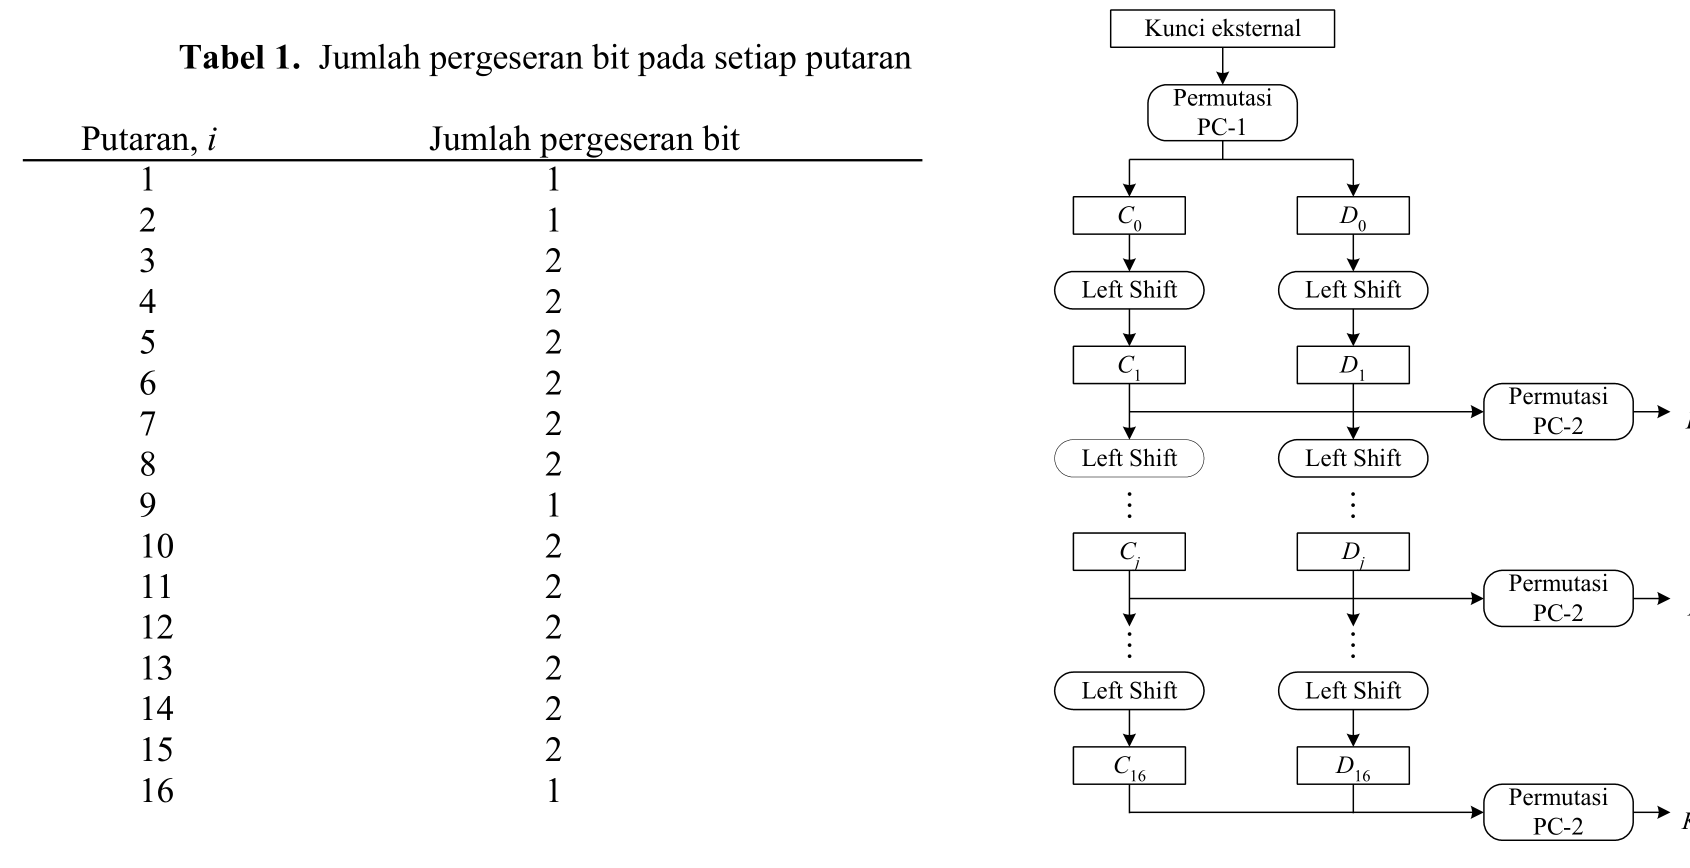
\includegraphics[width=184.80mm,height=238.79mm]{images/llm/page_014_img_01.png}%
\end{textblock*}

% bbox perkiraan otomatis: Diagram alir proses kriptografi yang menunjukkan langkah-langkah permutasi PC-1, pemisahan menjadi C dan D, operasi Left Shift berulang, dan permutasi PC-2 untuk menghasilkan kunci K1 hingga K16.

\newpage

% --- unit llm 15 ---
% === Halaman 15 (llm) ===

Matriks PC-2 berikut:

\vspace{20mm}

Jadi, $K_i$ merupakan penggabungan bit-bit $C_i$ pada posisi:
\[ 14, 17, 11, 24, 1, 5, 3, 28, 15, 6, 21, 10 \\
 23, 19, 12, 4, 26, 8, 16, 7, 27, 20, 13, 2 \]

dengan bit-bit $D_i$ pada posisi:
\[ 41, 52, 31, 37, 47, 55, 30, 40, 51, 45, 33, 48 \\
 44, 49, 39, 56, 34, 53, 46, 42, 50, 36, 29, 32 \]

Setiap kunci internal $K_i$ mempunyai panjang 48 bit.

% deskripsi: Tabel matriks permutasi PC-2 yang berisi angka-angka posisi bit.
% bbox normalisasi: [0.0330, 0.1350, 0.5910, 0.3250]
\begin{textblock*}{117.18mm}(6.93mm,40.10mm)
\noindent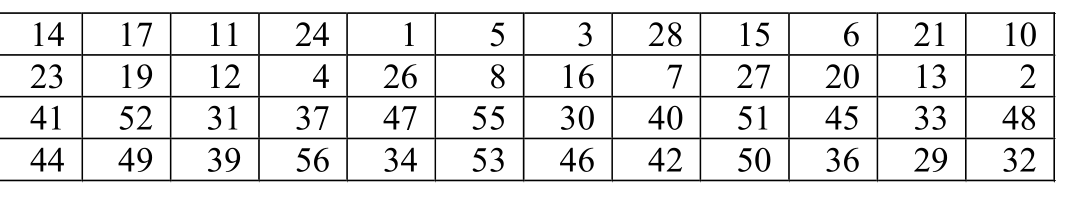
\includegraphics[width=117.18mm,height=56.43mm]{images/llm/page_015_img_01.png}%
\end{textblock*}

% deskripsi: Diagram alir proses pembangkitan kunci internal Ki menggunakan permutasi PC-1, operasi Left Shift pada register C dan D, serta permutasi PC-2.
% bbox normalisasi: [0.6550, 0.1350, 0.9600, 0.8450]
\begin{textblock*}{64.05mm}(137.55mm,40.10mm)
\noindent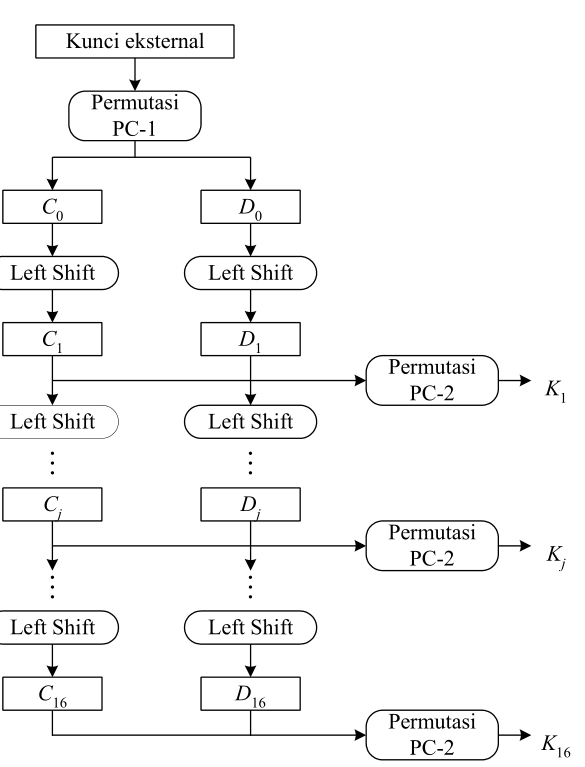
\includegraphics[width=64.05mm,height=210.87mm]{images/llm/page_015_img_02.png}%
\end{textblock*}

\newpage

% --- unit llm 16 ---
% === Halaman 16 (llm) ===

\vspace{196.02mm}

\begin{center}
\huge Pembangkitan kunci internal secara lengkap:
\end{center}

\vspace{80mm}

\begin{flushright}
Sumber: Cryptography\
and Network Security\
Chapter 3, Lecture slides\
by Lawrie Brown\
Modified by Richard\
Newman
\end{flushright}

% deskripsi: Diagram proses pembangkitan kunci internal (key schedule) yang menunjukkan permutasi, pergeseran (left shift), dan pemilihan bit untuk menghasilkan subkey 48-bit dari kunci 64-bit dengan bit paritas.
% bbox normalisasi: [0.0900, 0.1500, 0.9400, 0.8100]
\begin{textblock*}{178.50mm}(18.90mm,44.55mm)
\noindent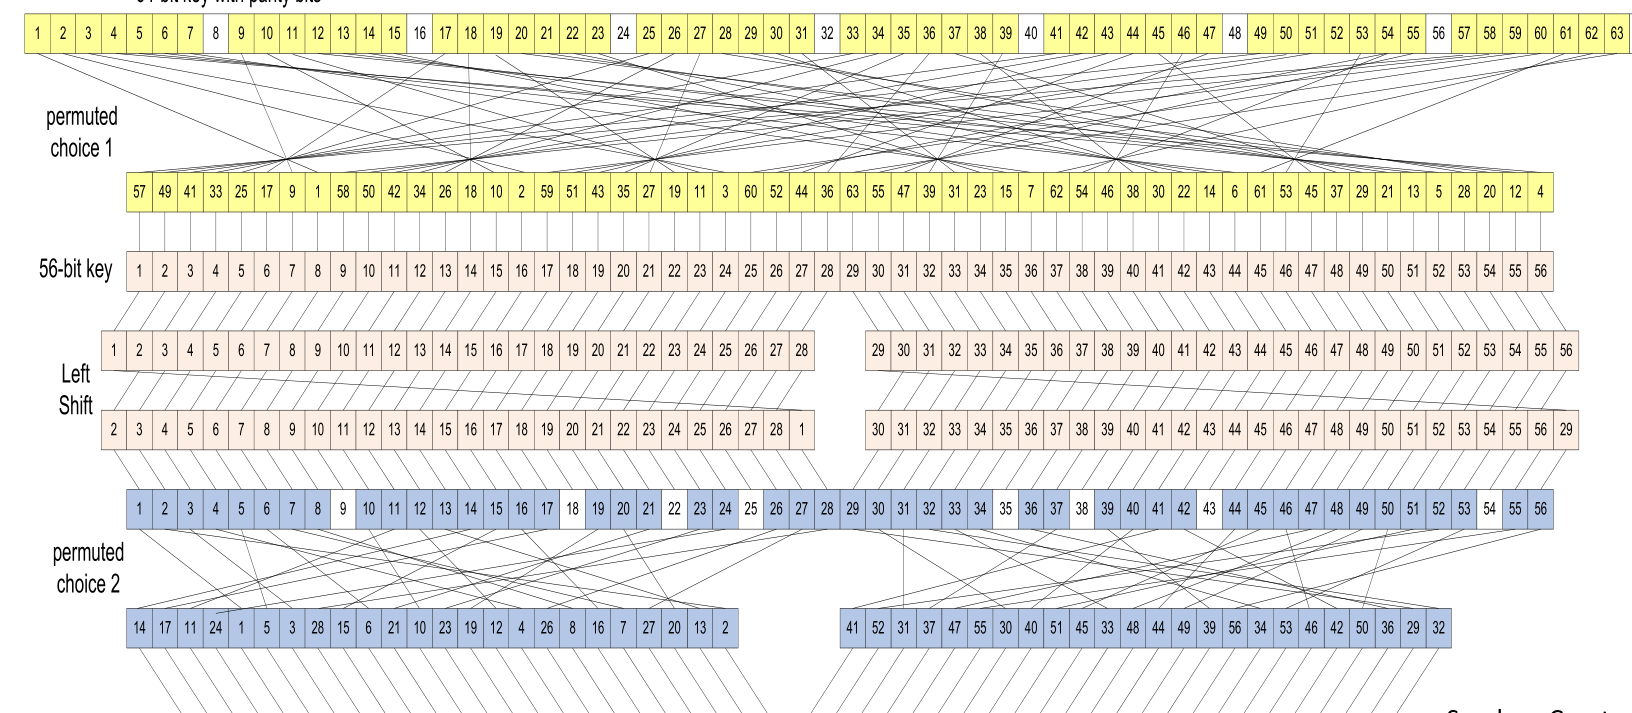
\includegraphics[width=178.50mm,height=196.02mm]{images/llm/page_016_img_01.png}%
\end{textblock*}

\newpage

% --- unit llm 17 ---
% === Halaman 17 (llm) ===

\section*{Permutasi Awal}

\vspace{86.13mm}

\begin{itemize}
    \item Tujuan: mengacak plainteks sehingga urutan bit-bit di dalamnya berubah.
    \item Matriks permutasi awal ($IP$):
\end{itemize}

\vspace{10mm}

\begin{tabular}{|c|c|c|c|c|c|c|c|c|c|c|c|c|c|c|c|}
\hline
58 & 50 & 42 & 34 & 26 & 18 & 10 & 2 & 60 & 52 & 44 & 36 & 28 & 20 & 12 & 4 \\ \hline
62 & 54 & 46 & 38 & 30 & 22 & 14 & 6 & 64 & 56 & 48 & 40 & 32 & 24 & 16 & 8 \\ \hline
57 & 49 & 41 & 33 & 25 & 17 & 9 & 1 & 59 & 51 & 43 & 35 & 27 & 19 & 11 & 3 \\ \hline
61 & 53 & 45 & 37 & 29 & 21 & 13 & 5 & 63 & 55 & 47 & 39 & 31 & 23 & 15 & 7 \\ \hline
\end{tabular}

% deskripsi: Diagram alur proses enkripsi yang melibatkan blok plainteks, tahap IP (Initial Permutation), proses Enciphering yang diulang 16 kali, dan tahap IP-1 (Inverse Initial Permutation) untuk menghasilkan blok cipherteks.
% bbox normalisasi: [0.7100, 0.2000, 0.9800, 0.4900]
\begin{textblock*}{56.70mm}(149.10mm,59.40mm)
\noindent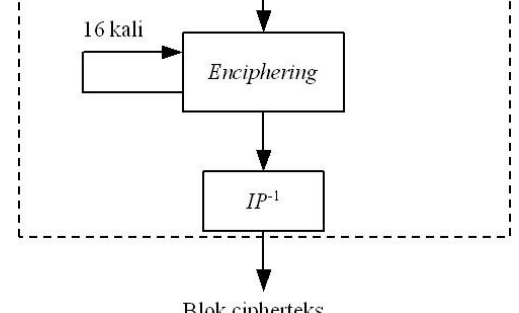
\includegraphics[width=56.70mm,height=86.13mm]{images/llm/page_017_img_01.png}%
\end{textblock*}

\newpage

% --- unit llm 18 ---
% === Halaman 18 (llm) ===

\vspace{95.04mm}

\section*{Enciphering}

\begin{itemize}
    \item Setiap blok plainteks mengalami 16 kali putaran \textit{enciphering}
    \item Setiap putaran \textit{enciphering} merupakan jaringan Feistel:
    \[
    \begin{aligned}
    L_i &= R_{i-1} \\
    R_i &= L_{i-1} \oplus f(R_{i-1}, K_i)
    \end{aligned}
    \]
\end{itemize}

\vspace{40mm}

\textbf{Gambar 4. Satu putaran \textit{enciphering}}

% deskripsi: Diagram alur proses enciphering secara keseluruhan yang melibatkan IP, 16 kali putaran enciphering, IP-1, dan key expansion.
% bbox normalisasi: [0.7200, 0.0000, 0.9800, 0.3200]
\begin{textblock*}{54.60mm}(151.20mm,0.00mm)
\noindent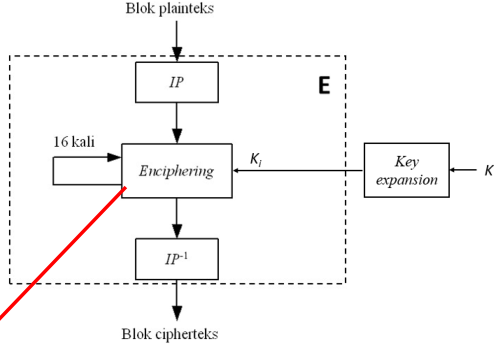
\includegraphics[width=54.60mm,height=95.04mm]{images/llm/page_018_img_01.png}%
\end{textblock*}

% deskripsi: Diagram detail satu putaran jaringan Feistel yang menunjukkan operasi XOR antara L_{i-1} dengan hasil fungsi f(R_{i-1}, K_i) untuk menghasilkan R_i, sementara R_{i-1} menjadi L_i.
% bbox normalisasi: [0.4000, 0.4400, 0.9300, 0.9000]
\begin{textblock*}{111.30mm}(84.00mm,130.68mm)
\noindent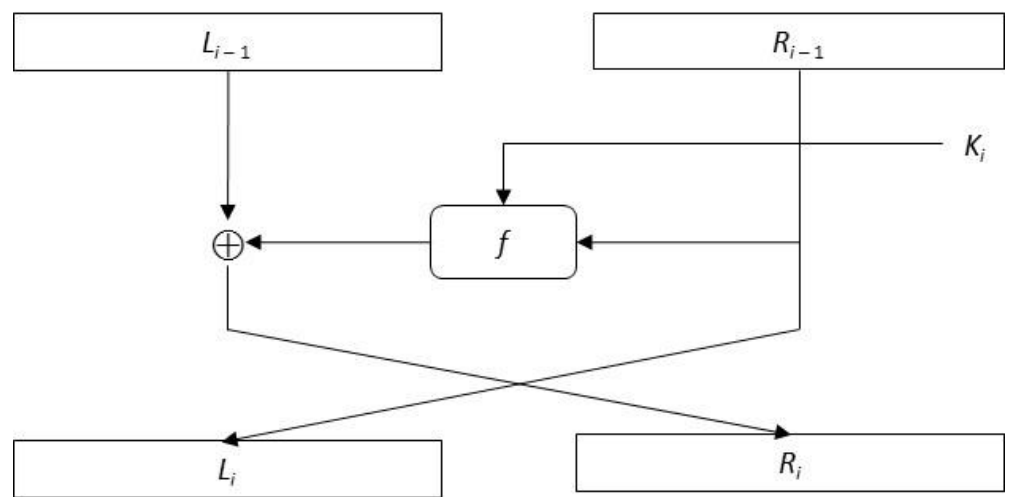
\includegraphics[width=111.30mm,height=136.62mm]{images/llm/page_018_img_02.png}%
\end{textblock*}

\newpage

% --- unit llm 19 ---
% === Halaman 19 (llm) ===

\vspace{273.24mm}

\vspace{10mm}
\textbf{Gambar 5. Diagram komputasi fungsi $f$:}

% deskripsi: Diagram alir komputasi fungsi f dalam algoritma DES, menunjukkan proses ekspansi, XOR dengan kunci, substitusi S-box, dan permutasi.
% bbox normalisasi: [0.0000, 0.0000, 0.9800, 0.9200]
\begin{textblock*}{205.80mm}(0.00mm,0.00mm)
\noindent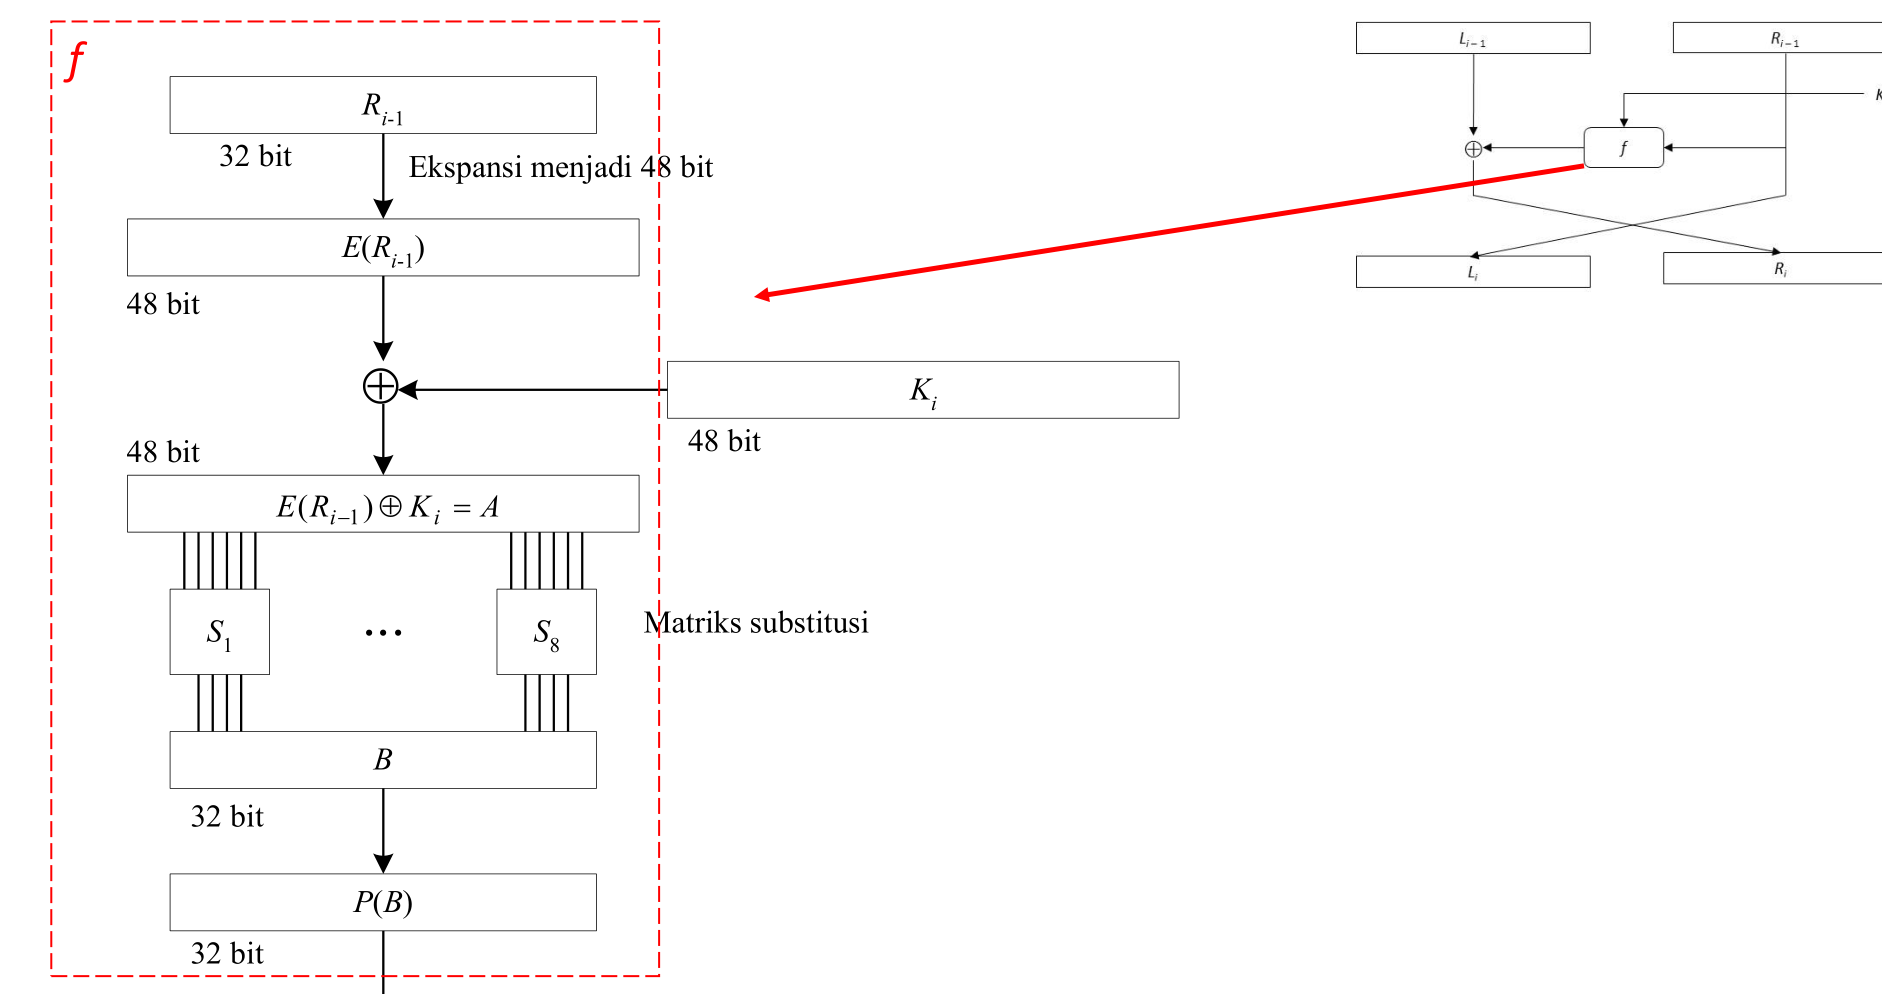
\includegraphics[width=205.80mm,height=273.24mm]{images/llm/page_019_img_01.png}%
\end{textblock*}

\newpage

% --- unit llm 20 ---
% === Halaman 20 (llm) ===

\vspace{231.66mm}

\begin{itemize}
    \item $E$ adalah fungsi ekspansi yang memperluas blok $R_{i-1}$ 32-bit menjadi blok 48 bit.
    \item Fungsi ekspansi direalisasikan dengan matriks permutasi ekspansi:
\end{itemize}

\begin{tabular}{|c|c|c|c|c|c|c|c|c|c|c|c|c|c|c|c|}
\hline
32 & 1 & 2 & 3 & 4 & 5 & 4 & 5 & 6 & 7 & 8 & 9 \\
\hline
8 & 9 & 10 & 11 & 12 & 13 & 12 & 13 & 14 & 15 & 16 & 17 \\
\hline
16 & 17 & 18 & 19 & 20 & 21 & 20 & 21 & 22 & 23 & 24 & 25 \\
\hline
24 & 25 & 26 & 27 & 28 & 29 & 28 & 29 & 30 & 31 & 32 & 1 \\
\hline
\end{tabular}

\vspace{20mm}

% deskripsi: Diagram alur proses enkripsi yang melibatkan fungsi ekspansi E, operasi XOR dengan kunci Ki, matriks substitusi S-box, dan permutasi P(B).
% bbox normalisasi: [0.6300, 0.1000, 0.9900, 0.8800]
\begin{textblock*}{75.60mm}(132.30mm,29.70mm)
\noindent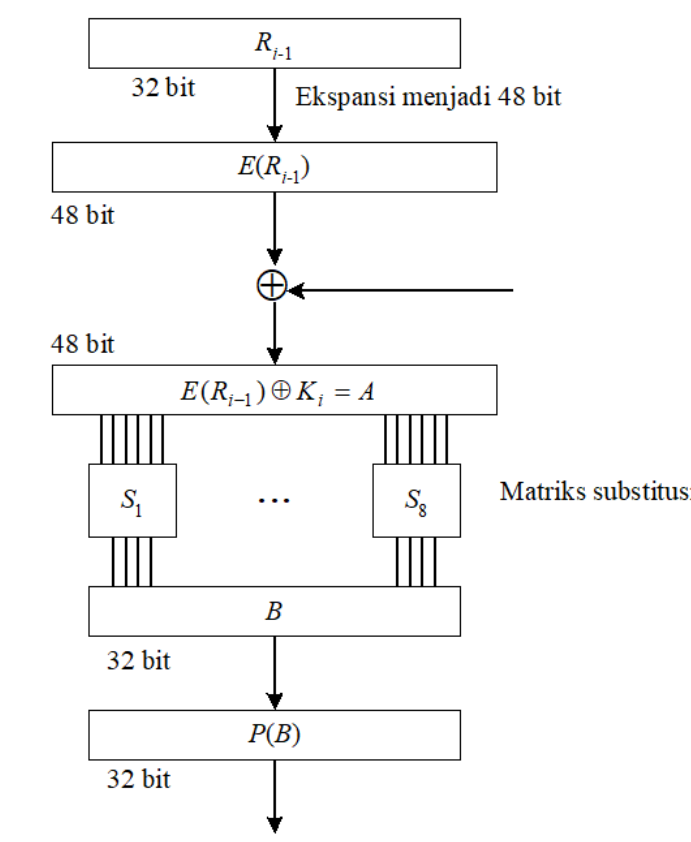
\includegraphics[width=75.60mm,height=231.66mm]{images/llm/page_020_img_01.png}%
\end{textblock*}

\newpage

% --- unit llm 21 ---
% === Halaman 21 (llm) ===

\vspace{196.02mm}

\begin{itemize}
    \item Hasil ekspansi, yaitu $E(R_{i-1})$ di-XOR-kan dengan $K_i$ menghasilkan blok A berukuran 48-bit:
    \[ E(R_{i-1}) \oplus K_i = A \]
    \vspace{50mm}
    \item Blok $A$ dikelompokkan menjadi 8 kelompok, masing-masing 6 bit, dan menjadi masukan bagi proses substitusi.
    \item Ada 8 matriks substitusi, masing-masing dinyatakan dengan kotak-S.
    \item Kotak-S menerima masukan 6 bit dan memberikan luaran 4 bit.
\end{itemize}

% deskripsi: Diagram alir proses enkripsi yang menunjukkan tahap ekspansi dari R_{i-1} (32 bit) menjadi 48 bit, operasi XOR dengan K_i untuk menghasilkan blok A, proses substitusi melalui kotak-S (S1 sampai S8), dan tahap permutasi P(B).
% bbox normalisasi: [0.5100, 0.2500, 0.9600, 0.9100]
\begin{textblock*}{94.50mm}(107.10mm,74.25mm)
\noindent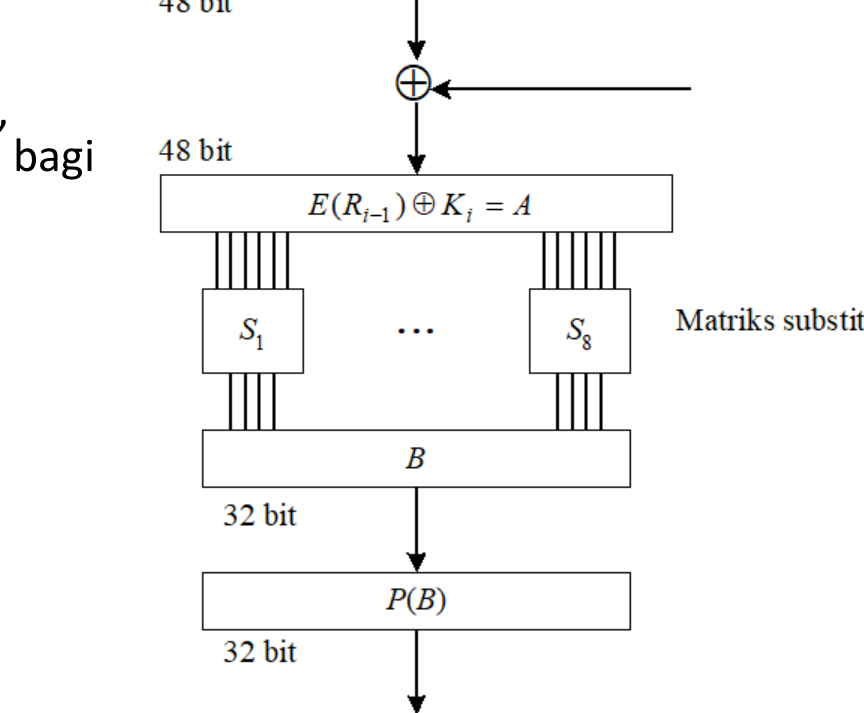
\includegraphics[width=94.50mm,height=196.02mm]{images/llm/page_021_img_01.png}%
\end{textblock*}

\newpage

% --- unit llm 22 ---
% === Halaman 22 (llm) ===

$S_1$:
\vspace{5mm}
$S_2$:
\vspace{5mm}
$S_3$:
\vspace{5mm}
$S_4$:

\vspace{38.61mm}

% deskripsi: Tabel matriks S1 berisi angka-angka acak dalam grid 4x15
% bbox normalisasi: [0.6600, 0.6600, 1.0000, 1.0000]
\begin{textblock*}{71.40mm}(138.60mm,196.02mm)
\noindent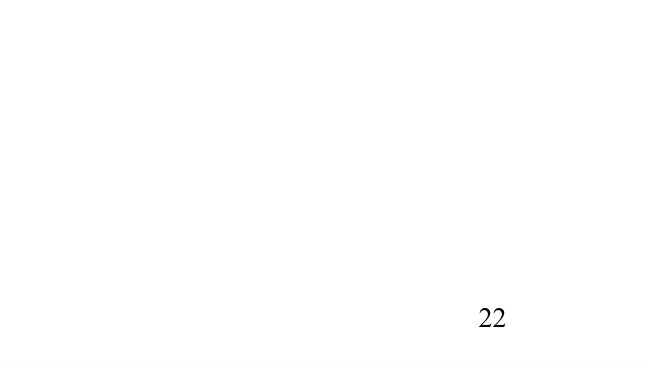
\includegraphics[width=71.40mm,height=100.98mm]{images/llm/page_022_img_01.png}%
\end{textblock*}

% deskripsi: Tabel matriks S2 berisi angka-angka acak dalam grid 4x15
% bbox normalisasi: [0.0400, 0.3000, 0.6400, 0.4400]
\begin{textblock*}{126.00mm}(8.40mm,89.10mm)
\noindent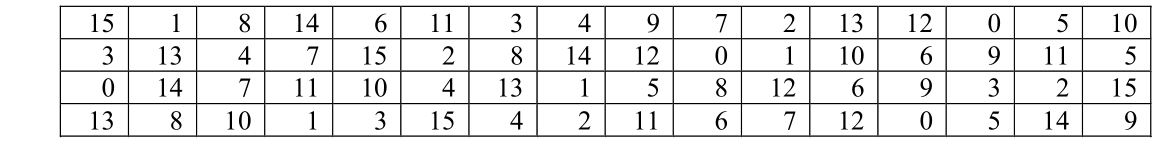
\includegraphics[width=126.00mm,height=41.58mm]{images/llm/page_022_img_02.png}%
\end{textblock*}

% deskripsi: Tabel matriks S3 berisi angka-angka acak dalam grid 4x15
% bbox normalisasi: [0.0400, 0.5200, 0.6400, 0.6500]
\begin{textblock*}{126.00mm}(8.40mm,154.44mm)
\noindent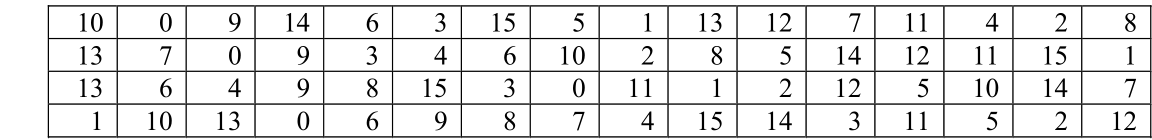
\includegraphics[width=126.00mm,height=38.61mm]{images/llm/page_022_img_03.png}%
\end{textblock*}

% deskripsi: Tabel matriks S4 berisi angka-angka acak dalam grid 4x15
% bbox normalisasi: [0.0400, 0.7300, 0.6400, 0.8600]
\begin{textblock*}{126.00mm}(8.40mm,216.81mm)
\noindent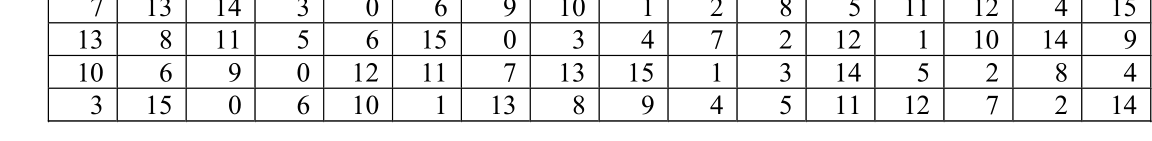
\includegraphics[width=126.00mm,height=38.61mm]{images/llm/page_022_img_04.png}%
\end{textblock*}

\newpage

% --- unit llm 23 ---
% === Halaman 23 (llm) ===

\vspace{264.33mm}

Input: $\text{101010}$
Baris = $\text{10} = 2$
Kolom = $\text{0101} = 5$
Luaran = $13 = 1101$

\vspace{50mm}

\begin{itemize}
    \item Setiap baris di dalam S-box adalah permutasi angka-angka $0, 1, 2, \dots, 15$.
    \item Mengubah satu bit di dalam input S-box mengakibatkan perubahan paling sedikit 2 bit pada output S-box
\end{itemize}

$\rightarrow$ prinsip \textit{confussion}

% deskripsi: Empat tabel S-box ($S_5, S_6, S_7, S_8$) yang digunakan dalam proses substitusi kriptografi, dengan tabel $S_5$ menunjukkan proses indexing baris dan kolom.
% bbox normalisasi: [0.2100, 0.0000, 0.9200, 0.8900]
\begin{textblock*}{149.10mm}(44.10mm,0.00mm)
\noindent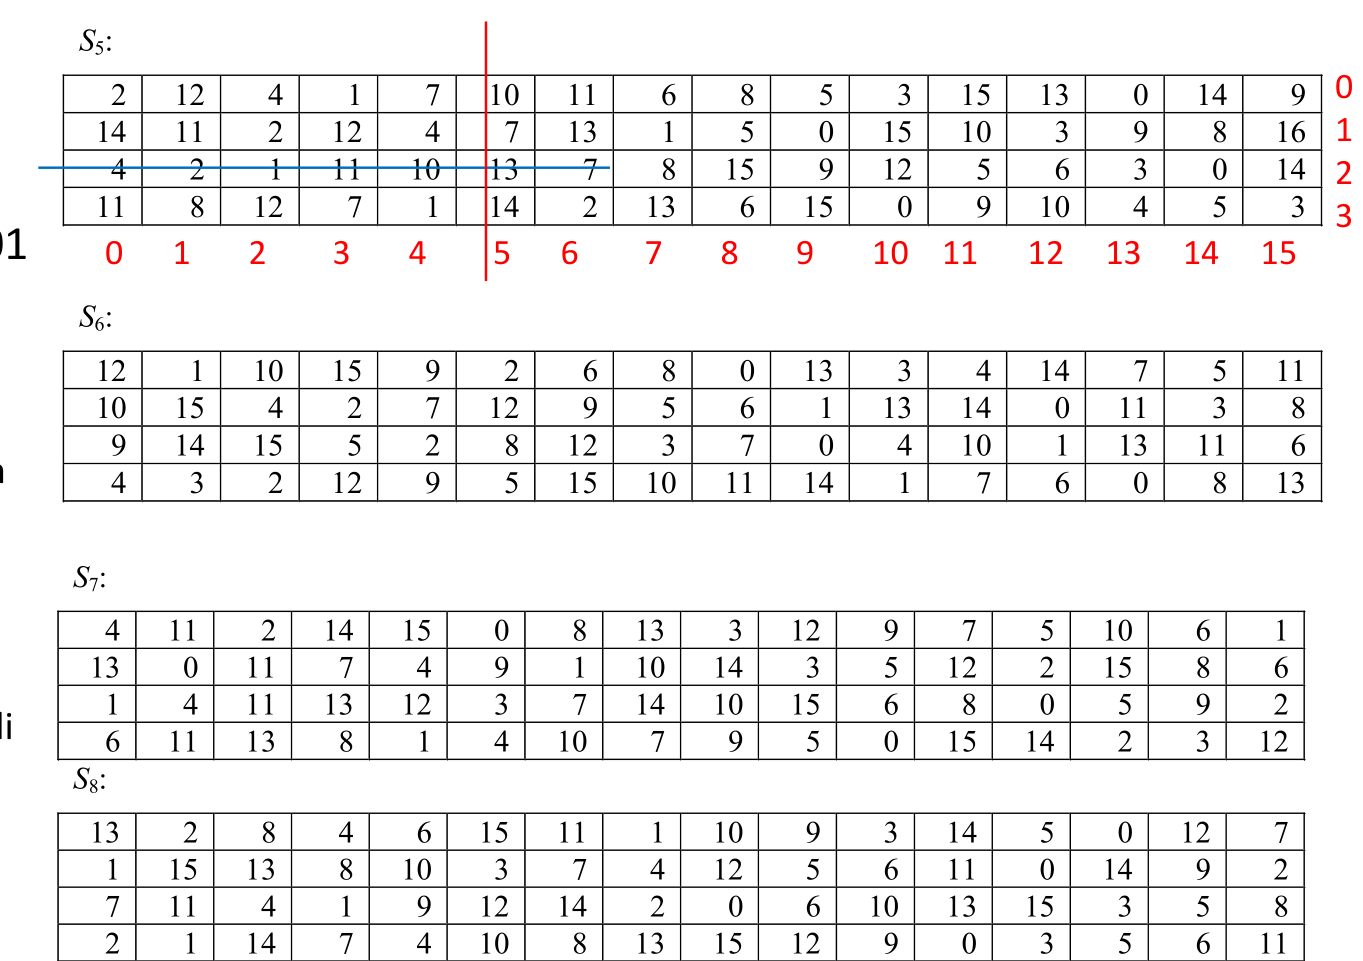
\includegraphics[width=149.10mm,height=264.33mm]{images/llm/page_023_img_01.png}%
\end{textblock*}

\newpage

% --- unit llm 24 ---
% === Halaman 24 (llm) ===

\begin{itemize}
  \item Luaran proses substitusi adalah blok $B$ yang panjangnya 32 bit.
  \item Blok $B$ menjadi masukan untuk proses permutasi.
  \item Tujuan permutasi adalah untuk mengacak hasil proses substitusi kotak-S.
  \item Permutasi dilakukan dengan menggunakan matriks permutasi $P$ (P-box) sbb:
\end{itemize}

\vspace{10mm}

\begin{center}
\begin{tabular}{|c|c|c|c|c|c|c|c|c|c|c|c|c|c|c|c|}
\hline
16 & 7 & 20 & 21 & 29 & 12 & 28 & 17 & 1 & 15 & 23 & 26 & 5 & 8 & 31 & 10 \\ \hline
2 & 8 & 24 & 14 & 32 & 27 & 3 & 9 & 19 & 13 & 30 & 6 & 22 & 11 & 4 & 25 \\ \hline
\end{tabular}
\end{center}

% deskripsi: Diagram alur proses kriptografi yang menunjukkan langkah-langkah dari input R_{i-1}, ekspansi menjadi 48 bit, fungsi E, operasi XOR dengan K_i menghasilkan A, substitusi melalui S-box menjadi blok B, dan terakhir proses permutasi P(B).
% bbox normalisasi: [0.6600, 0.6000, 0.9900, 0.8300]
\begin{textblock*}{69.30mm}(138.60mm,178.20mm)
\noindent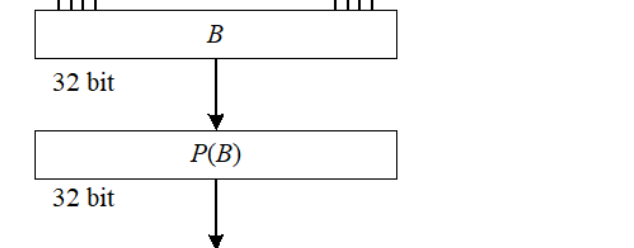
\includegraphics[width=69.30mm,height=68.31mm]{images/llm/page_024_img_01.png}%
\end{textblock*}

\newpage

% --- unit llm 25 ---
% === Halaman 25 (llm) ===

\vspace{138.11mm}

\begin{itemize}
    \item $P(B)$ merupakan luaran dari fungsi $f$.
    \item Bit-bit $P(B)$ di-XOR-kan dengan $L_{i-1}$ menghasilkan $R_i$:
    \[ R_i = L_{i-1} \oplus P(B) \]
    \item Jadi, luaran dari putaran ke-$i$ adalah
    \[ (L_i, R_i) = (R_{i-1}, L_{i-1} \oplus P(B)) \]
\end{itemize}
\vspace{10mm}

% deskripsi: Diagram alur logika yang menunjukkan operasi XOR antara input L_{i-1} (32 bit) dan output fungsi f untuk menghasilkan R_i (32 bit).
% bbox normalisasi: [0.4630, 0.4180, 0.9330, 0.8830]
\begin{textblock*}{98.70mm}(97.23mm,124.15mm)
\noindent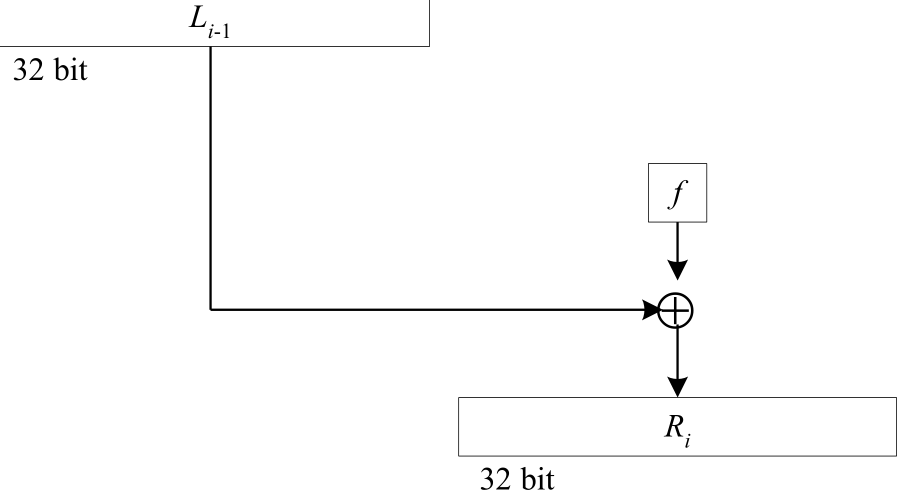
\includegraphics[width=98.70mm,height=138.11mm]{images/llm/page_025_img_01.png}%
\end{textblock*}

\newpage

% --- unit llm 26 ---
% === Halaman 26 (llm) ===

\vspace{100.98mm}

\section*{Inversi Permutasi ($\text{IP}^{-1}$)}

\begin{itemize}
    \item Permutasi terakhir dilakukan setelah 16 kali putaran terhadap gabungan blok kiri dan blok kanan.
    \item Permutasi menggunakan matriks permutasi awal balikan ($\text{IP}^{-1}$) sbb:
\end{itemize}

\vspace{10mm}

\begin{tabular}{|c|c|c|c|c|c|c|c|c|c|c|c|c|c|c|c|}
\hline
40 & 8 & 48 & 16 & 56 & 24 & 64 & 32 & 39 & 7 & 47 & 15 & 55 & 23 & 63 & 31 \\ \hline
38 & 6 & 46 & 14 & 54 & 22 & 62 & 30 & 37 & 5 & 45 & 13 & 53 & 21 & 61 & 29 \\ \hline
36 & 4 & 44 & 12 & 52 & 20 & 60 & 28 & 35 & 3 & 43 & 11 & 51 & 19 & 59 & 27 \\ \hline
34 & 2 & 42 & 10 & 50 & 18 & 58 & 26 & 33 & 1 & 41 & 9 & 49 & 17 & 57 & 25 \\ \hline
\end{tabular}

% deskripsi: Diagram alur proses enkripsi DES yang menunjukkan langkah-langkah dari blok plaintext, Initial Permutation (IP), 16 kali putaran Enciphering dengan Key expansion, hingga Inverse Initial Permutation (IP-1) untuk menghasilkan blok ciphertext.
% bbox normalisasi: [0.7100, 0.0000, 0.9900, 0.3400]
\begin{textblock*}{58.80mm}(149.10mm,0.00mm)
\noindent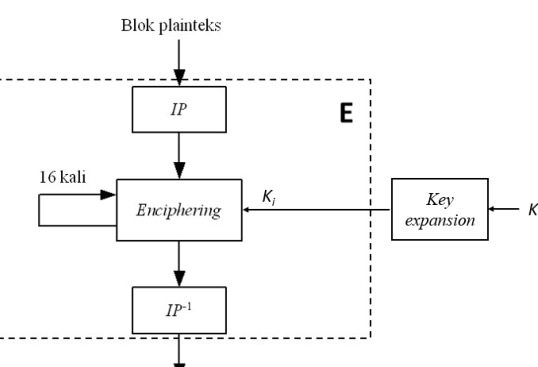
\includegraphics[width=58.80mm,height=100.98mm]{images/llm/page_026_img_01.png}%
\end{textblock*}

\newpage

% --- unit llm 27 ---
% === Halaman 27 (llm) ===

\vspace{225.72mm}

Satu putaran di dalam DES:

% deskripsi: Diagram alur satu putaran (round) dalam algoritma enkripsi DES, menunjukkan proses pengolahan L, R, C, dan D dengan fungsi F, XOR, S-box, dan permutasi.
% bbox normalisasi: [0.1700, 0.1800, 0.7600, 0.9400]
\begin{textblock*}{123.90mm}(35.70mm,53.46mm)
\noindent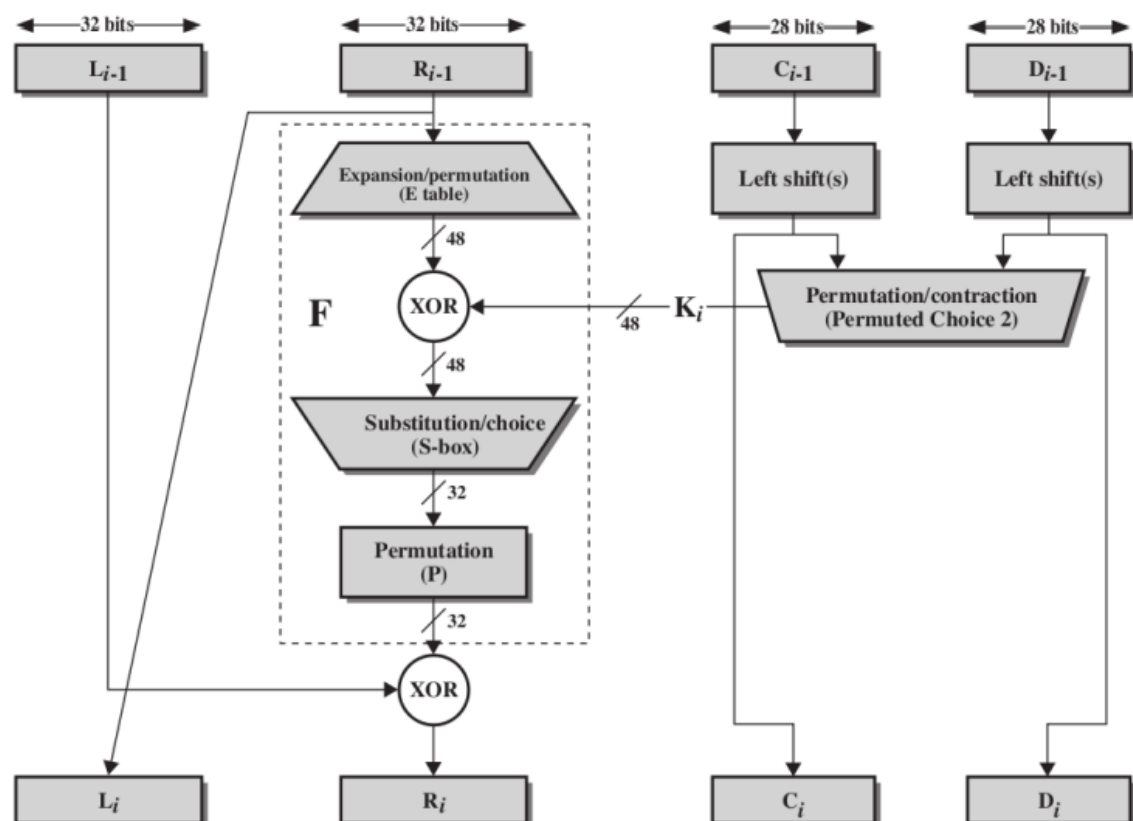
\includegraphics[width=123.90mm,height=225.72mm]{images/llm/page_027_img_01.png}%
\end{textblock*}

\newpage

% --- unit llm 28 ---
% === Halaman 28 (llm) ===

\vspace{246.51mm}

\section*{Satu putaran di dalam jaringan Feistel secara lengkap:}

\vspace{100mm}

Sumber: Cryptography and Network Security \\
Chapter 3, Lecture slides by Lawrie Brown \\
Modified by Richard Newman

% deskripsi: Diagram blok tingkat tinggi dari satu putaran jaringan Feistel yang menunjukkan operasi XOR dan fungsi f.
% bbox normalisasi: [0.7090, 0.0000, 0.9960, 0.2300]
\begin{textblock*}{60.27mm}(148.89mm,0.00mm)
\noindent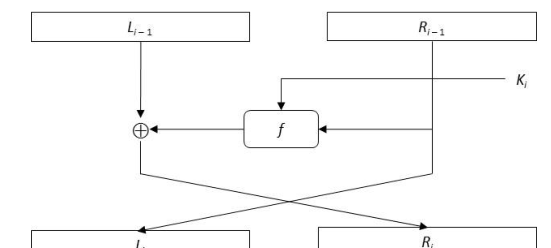
\includegraphics[width=60.27mm,height=68.31mm]{images/llm/page_028_img_01.png}%
\end{textblock*}

% deskripsi: Diagram alur mendetail dari satu putaran jaringan Feistel, menunjukkan permutasi bit, input simbol, S-box (S1-S8), dan ekspansi bit.
% bbox normalisasi: [0.0000, 0.1300, 0.9960, 0.9600]
\begin{textblock*}{209.16mm}(0.00mm,38.61mm)
\noindent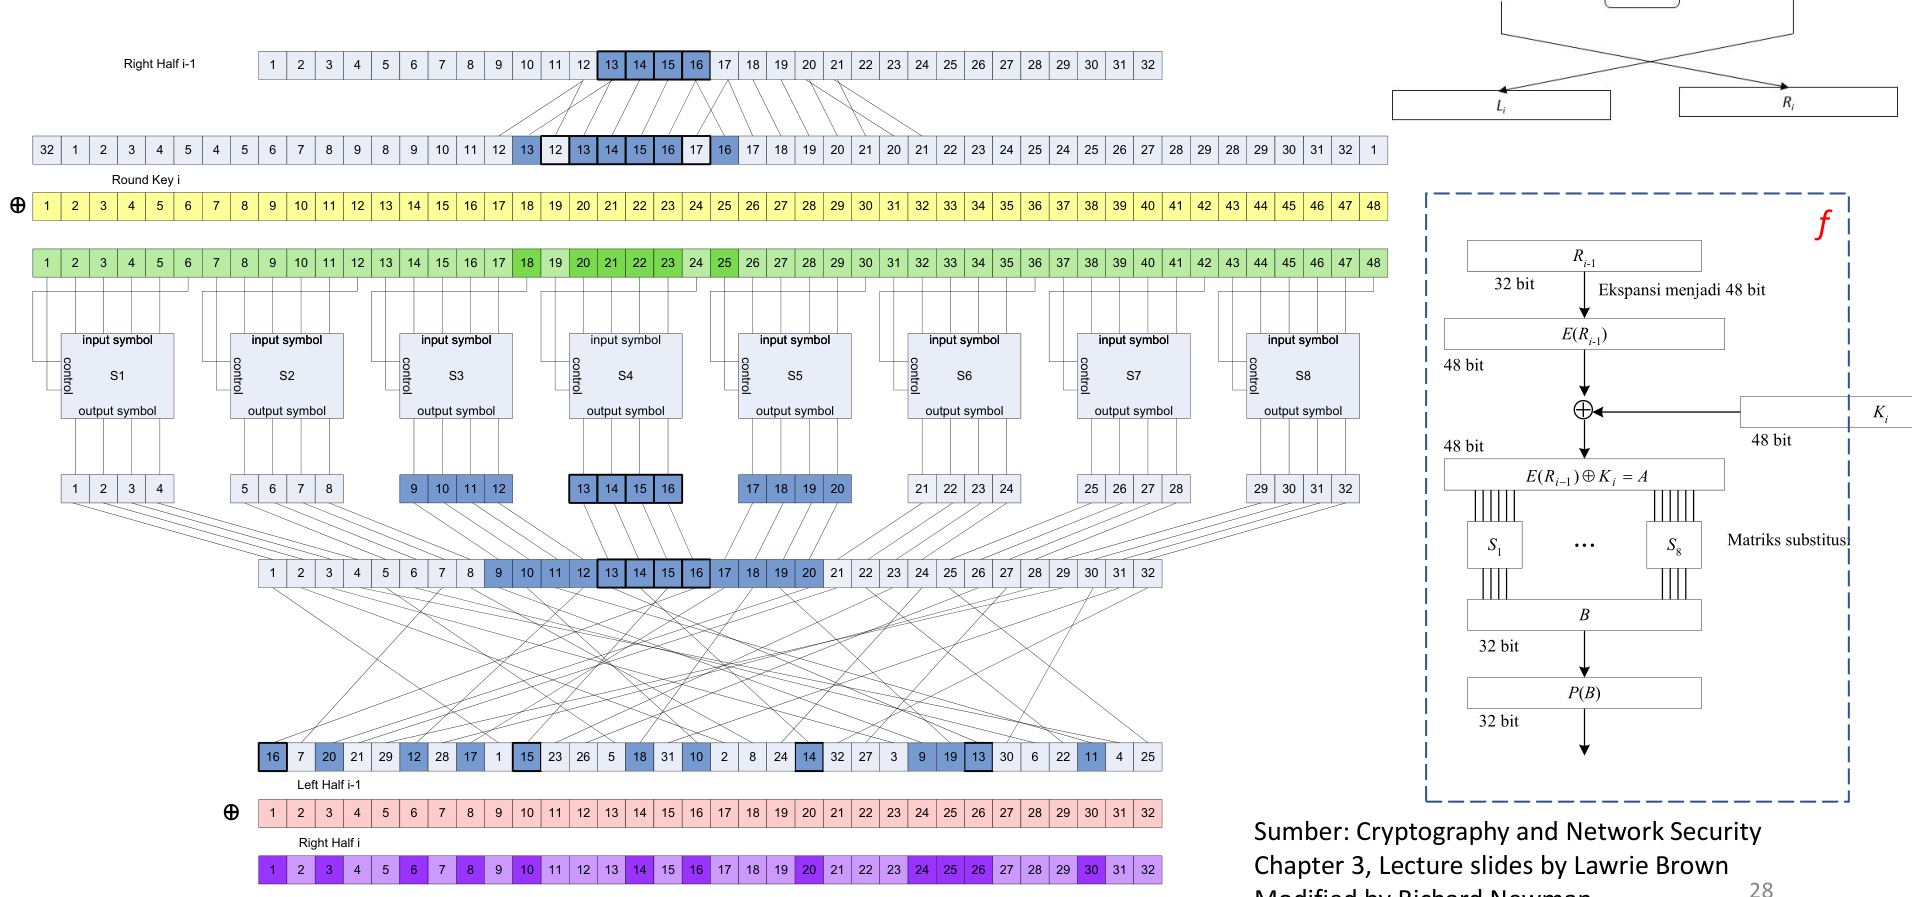
\includegraphics[width=209.16mm,height=246.51mm]{images/llm/page_028_img_02.png}%
\end{textblock*}

% deskripsi: Diagram detail internal fungsi f dalam jaringan Feistel, menunjukkan ekspansi, operasi XOR dengan kunci Ki, matriks substitusi S-box, dan permutasi P.
% bbox normalisasi: [0.7130, 0.2800, 0.9960, 0.8300]
\begin{textblock*}{59.43mm}(149.73mm,83.16mm)
\noindent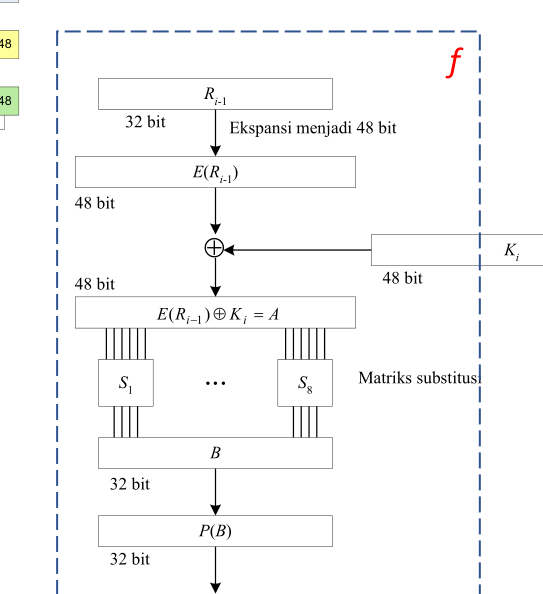
\includegraphics[width=59.43mm,height=163.35mm]{images/llm/page_028_img_03.png}%
\end{textblock*}

\newpage

% --- unit llm 29 ---
% === Halaman 29 (llm) ===

\vspace{243.54mm}

Contoh hasil enkripsi DES pada setiap putaran:

\vspace{20mm}

Sumber: Cryptography and Network Security \\ Chapter 3, Lecture slides by Lawrie Brown \\ Modified by Richard Newman

% deskripsi: Tabel yang menunjukkan hasil enkripsi DES untuk setiap putaran, mencakup kolom Round, K_i (kunci putaran), L_i (setengah kiri), dan R_i (setengah kanan) dari tahap IP hingga IP^-1.
% bbox normalisasi: [0.2400, 0.1300, 0.7200, 0.9500]
\begin{textblock*}{100.80mm}(50.40mm,38.61mm)
\noindent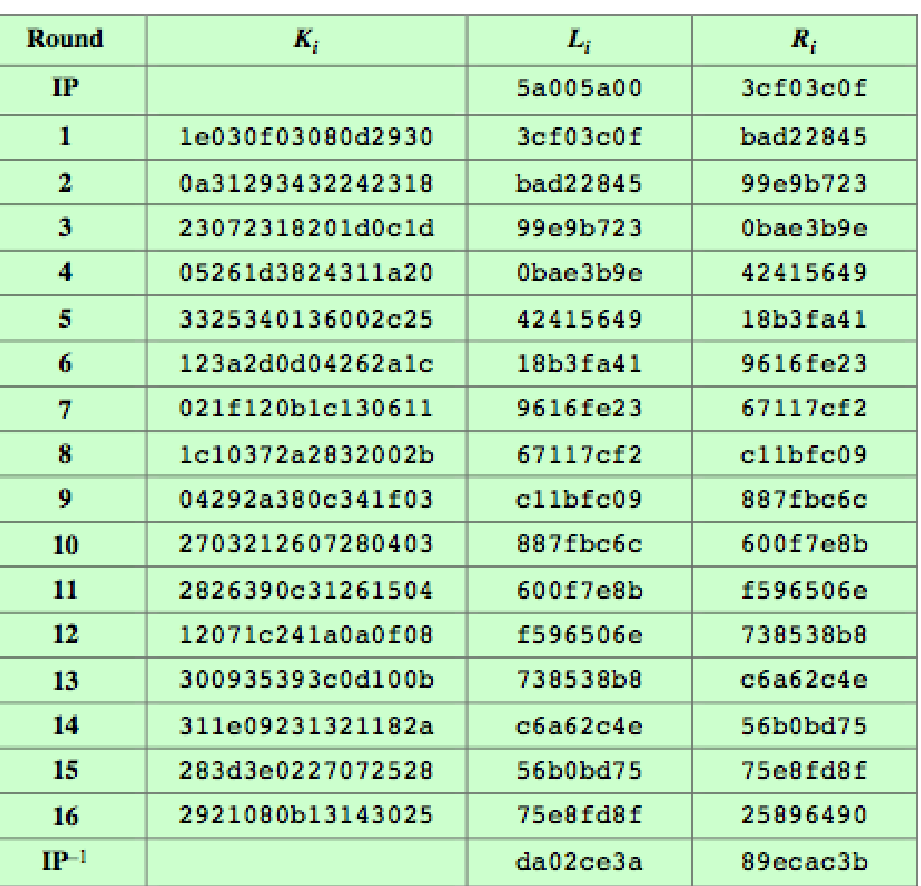
\includegraphics[width=100.80mm,height=243.54mm]{images/llm/page_029_img_01.png}%
\end{textblock*}

\newpage

% --- unit llm 30 ---
% === Halaman 30 (llm) ===

\section*{Dekripsi}

\begin{itemize}
    \item Dekripsi terhadap cipherteks merupakan kebalikan dari proses enkripsi.
    \item DES menggunakan algoritma yang sama untuk proses enkripsi dan dekripsi.
    \item Pada proses dekripsi urutan kunci yang digunakan adalah $K_{16}, K_{15}, \dots, K_1$.
    \item Untuk tiap putaran $16, 15, \dots, 1$, luaran pada setiap putaran \textit{deciphering} adalah
    \[
    \begin{aligned}
    R_{i-1} &= L_i \\
    L_{i-1} &= R_i \oplus f(R_{i-1}, K_i) = R_i \oplus f(L_i, K_i)
    \end{aligned}
    \]
\end{itemize}

\newpage

% --- unit llm 31 ---
% === Halaman 31 (llm) ===

Dekripsi:

\vspace{60mm}

\begin{align*}
R_{i-1} &= L_i \\
L_{i-1} &= R_i \oplus f(R_{i-1}, K_i) = R_i \oplus f(L_i, K_i)
\end{align*}

% deskripsi: Diagram alur proses dekripsi Feistel cipher yang menunjukkan hubungan antara L, R, fungsi f, dan kunci K.
% bbox normalisasi: [0.1300, 0.1900, 0.8400, 0.7900]
\begin{textblock*}{149.10mm}(27.30mm,56.43mm)
\noindent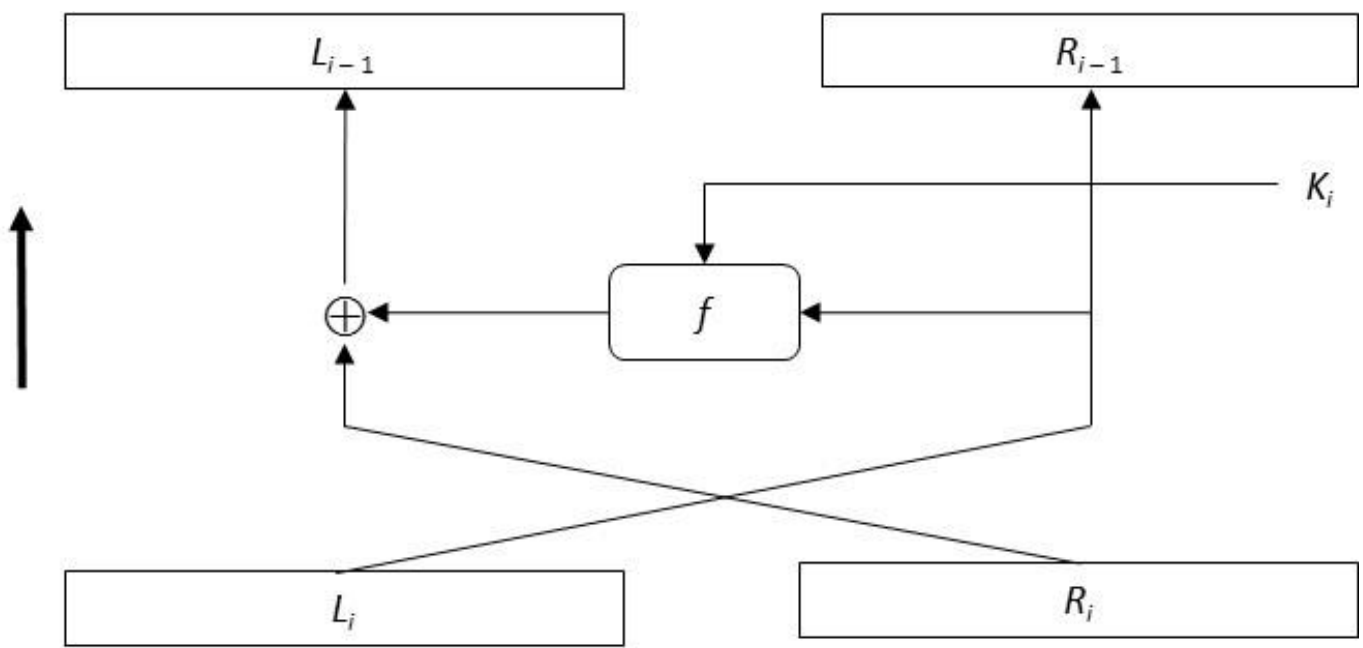
\includegraphics[width=149.10mm,height=178.20mm]{images/llm/page_031_img_01.png}%
\end{textblock*}

\newpage

% --- unit llm 32 ---
% === Halaman 32 (llm) ===

\section*{Efek longsoran (avalanche effect)}

\begin{itemize}
    \item Efek longsoran adalah properti kunci yang diinginkan dari algoritma enkripsi,
    \item Tujuan: menunjukkan perubahan satu bit pada plainteks atau kunci menghasilkan perubahan besar pada cipherteks
    \item Efek longsoran membuat upaya untuk mencoba menebak kunci menjadi tidak mungkin
    \item DES menunjukkan efek longsoran yang kuat
\end{itemize}

\newpage

% --- unit llm 33 ---
% === Halaman 33 (llm) ===

\begin{center}
\Huge Efek longsoran di dalam DES \\
\large (mengubah satu bit plainteks)
\end{center}

\vspace{50mm}

Sumber: Cryptography and Network Security \\
Chapter 3, Lecture slides by Lawrie Brown \\
Modified by Richard Newman

\vspace{20mm}

\begin{flushright}
Keterangan: \\
$\delta = $ jumlah perbedaan bit pada ciphertexts
\end{flushright}

% deskripsi: Tabel yang menunjukkan efek avalanche (longsoran) dalam DES, membandingkan ciphertexts dari plainteks original dan modified melalui berbagai round, serta menghitung perbedaan bit (delta).
% bbox normalisasi: [0.1470, 0.2240, 0.7100, 0.9320]
\begin{textblock*}{118.23mm}(30.87mm,66.53mm)
\noindent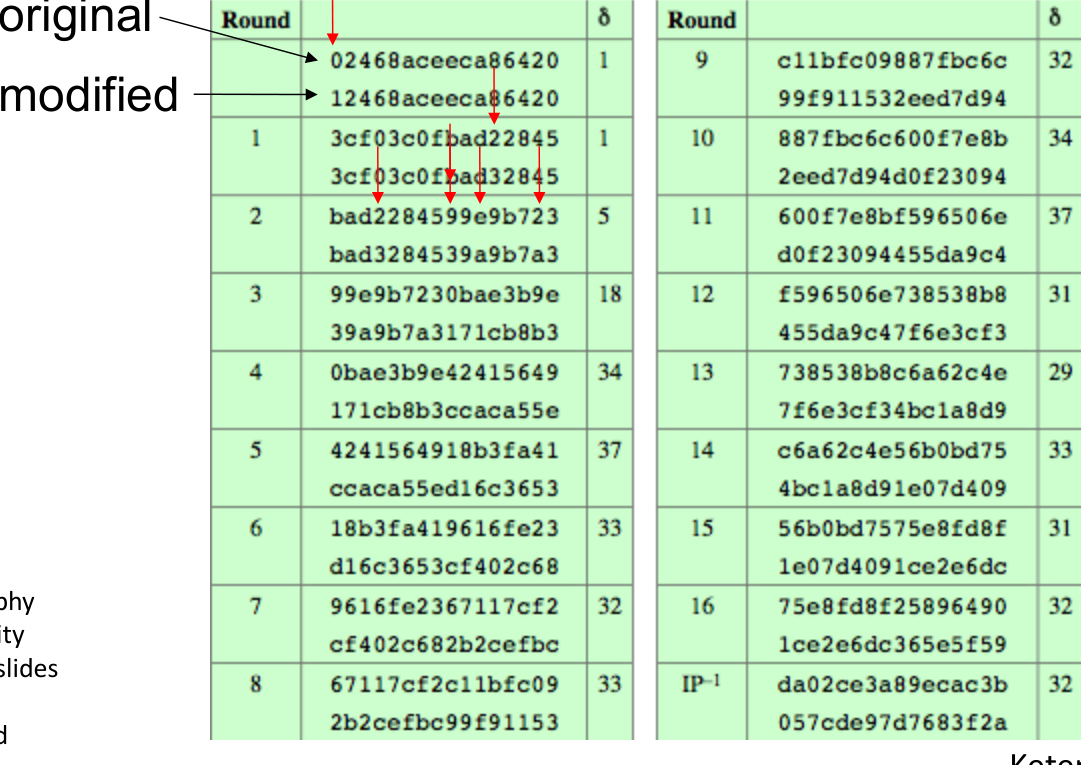
\includegraphics[width=118.23mm,height=210.28mm]{images/llm/page_033_img_01.png}%
\end{textblock*}

\newpage

% --- unit llm 34 ---
% === Halaman 34 (llm) ===

\vspace{231.07mm}

\begin{center}
\Huge Efek longsoran di dalam DES \\
\Large (mengubah satu bit kunci)
\end{center}

\vspace{10mm}

% deskripsi: Tabel yang menunjukkan efek longsoran (avalanche effect) pada algoritma DES, membandingkan nilai state internal antar round ketika satu bit kunci diubah, disertai dengan nilai delta ($\delta$) yang mengukur perbedaan bit.
% bbox normalisasi: [0.1930, 0.1850, 0.7430, 0.9630]
\begin{textblock*}{115.50mm}(40.53mm,54.95mm)
\noindent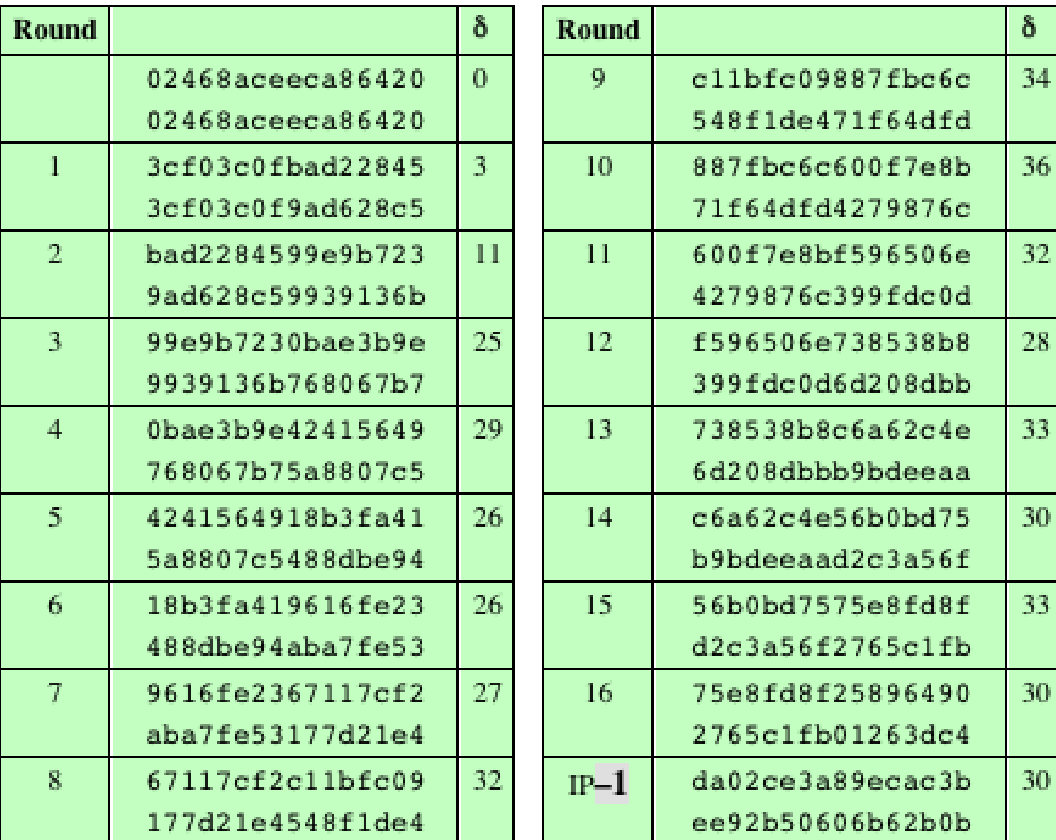
\includegraphics[width=115.50mm,height=231.07mm]{images/llm/page_034_img_01.png}%
\end{textblock*}

\newpage

% --- unit llm 35 ---
% === Halaman 35 (llm) ===

\section*{Mode DES}

\begin{itemize}
    \item DES dapat dioperasikan dengan mode ECB, CBC, OFB, CFB, dan mode \textit{counter}.
    \item Namun karena kesederhanaannya, mode ECB lebih sering digunakan pada paket komersil, sehingga dikenal dengan nama DES-ECB.
\end{itemize}

\newpage

% --- unit llm 36 ---
% === Halaman 36 (llm) ===

\section*{Kunci-kunci lemah DES}

\vspace{130.68mm}

\begin{itemize}
    \item \textbf{Kunci lemah DES} adalah kunci K sedemikian sehingga $E_K(E_K(x)) = x$ untuk semua plainteks x, yang artinya enkripsi dan dekripsi menjadi sama.
    \begin{itemize}
        \item Kunci lemah ini menghasilkan pembangkitan kunci putaran yang sama pada semua putaran.
    \end{itemize}
\end{itemize}

\begin{itemize}
    \item DES memiliki 4 kunci lemah (masing-masing panjangnya 56 bit), dinyatakan dalam kode heksadesimal sbb:
    \begin{align*}
        &0000000000000000 \\
        &0000000FFFFFFFF \\
        &FFFFFFF00000000 \\
        &FFFFFFFFFFFFFFFF
    \end{align*}
    \vspace{10mm}
    \item Kunci lemah seharusnya dihindari.
\end{itemize}

% deskripsi: Ilustrasi dua buah kunci berwarna kuning yang terikat pada satu gantungan kunci
% bbox normalisasi: [0.6500, 0.4700, 0.8550, 0.9100]
\begin{textblock*}{43.05mm}(136.50mm,139.59mm)
\noindent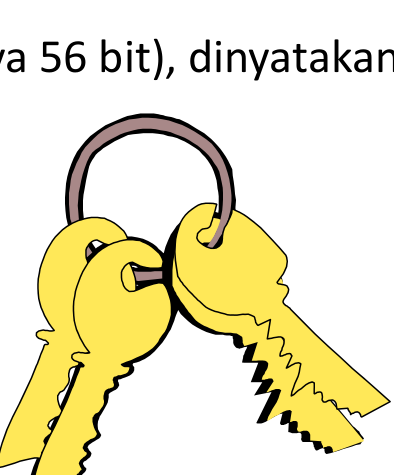
\includegraphics[width=43.05mm,height=130.68mm]{images/llm/page_036_img_01.png}%
\end{textblock*}

\newpage

% --- unit llm 37 ---
% === Halaman 37 (llm) ===

\section*{Implementasi DES}

\begin{itemize}
    \item DES sudah diimplementasikan baik sebagai perangkat lunak maupun perangkat keras.
    \item Dalam bentuk perangkat keras, DES diimplementasikan di dalam \textit{chip}. Setiap detik \textit{chip} ini dapat mengenkripsikan 16,8 juta blok (atau 1 gigabit per detik).
    \item Implementasi DES ke dalam perangkat lunak dapat melakukan enkripsi 32.000 blok per detik (dijalankan pada komputer \textit{mainframe} IBM 3090, yaitu komputer tercepat saat itu / tahun 1976).
\end{itemize}

\newpage

% --- unit llm 38 ---
% === Halaman 38 (llm) ===

\section*{Keamanan DES}

\begin{itemize}
    \item Keamanan DES ditentukan oleh kunci.
    \item Panjang kunci eksternal DES hanya 64 bit, tetapi yang dipakai hanya 56 bit.
    \item Pada rancangan awal, panjang kunci yang diusulkan IBM adalah 128 bit, tetapi atas permintaan NSA, panjang kunci diperkecil menjadi 56 bit.
    \item Dengan panjang kunci 56 bit akan terdapat $2^{56}$ atau 72.057.594.037.927.936 kemungkinan kunci.
    \item Ruang kunci (\textit{key space}) DES sebanyak $2^{56}$ terlalu kecil, tidak aman karena kunci dapat ditemukan dengan serangan \textit{exhaustive key search} (\textit{brute force attack})
    \item Jika serangan \textit{exhaustive key search} (\textit{brute force attack}) dengan menggunakan prosesor paralel, andaikan dalam satu detik dapat dikerjakan satu juta serangan. Jadi seluruhnya diperlukan 1142 tahun untuk menemukan kunci yang benar.
\end{itemize}

\newpage

% --- unit llm 39 ---
% === Halaman 39 (llm) ===

\begin{itemize}
    \item Misalkan kita mengetahui pasangan potongan plaintext ($p$) dan cipherteks ($c$) yang berkoresponden.
    \item Lakukan serangan \textit{brute force} (atau \textit{exhaustive key search attack}) dengan mencoba semua kemungkinan kunci ($k$):
\end{itemize}

\vspace{5mm}

\begin{verbatim}
for (k=0; k<2^{56}; k++) {
    if (DES(k, p) == c) {
        printf("Key is %x\n", k);
        break;
    }
}
\end{verbatim}

\vspace{5mm}

\begin{itemize}
    \item Kunci diharapkan ditemukan sebelum $2^{55}$ iterasi.
\end{itemize}

\newpage

% --- unit llm 40 ---
% === Halaman 40 (llm) ===

Dikutip dari Wiki:\
\begin{itemize}
    \item In 1997, RSA Security sponsored a series of contests, offering a \$10,000 prize to the first team that broke a message encrypted with DES for the contest.
    \item That contest was won by the DESCHALL Project, led by Rocke Verser, Matt Curtin, and Justin Dolske, using idle cycles of thousands of computers across the Internet.
\end{itemize}

\newpage

% --- unit llm 41 ---
% === Halaman 41 (llm) ===

\begin{itemize}
    \item Tahun 1998, \textit{Electronic Frontier Foundation} (EFE) merancang dan membuat perangkat keras khusus untuk menemukan kunci DES secara \textit{exhaustive key search} dengan biaya \$250.000 dan diharapkan dapat menemukan kunci selama 5 hari.
    \item Tahun 1999, kombinasi perangkat keras \textit{EFE} dengan kolaborasi internet yang melibatkan lebih dari 100.000 komputer dapat menemukan kunci DES kurang dari 1 hari.
\end{itemize}

\newpage

% --- unit llm 42 ---
% === Halaman 42 (llm) ===

\vspace{50mm}

The \href{https://www.eff.org}{EFF}'s US\$250,000 \href{https://en.wikipedia.org/wiki/DEScracker}{DES cracking machine} contained 1,856 custom chips and could brute force a DES key in a matter of days -- the photo shows a DES Cracker circuit board fitted with several Deep Crack chips (Sumber Wikipedia).

% deskripsi: Foto papan sirkuit DES Cracker yang dilengkapi dengan beberapa chip Deep Crack.
% bbox normalisasi: [0.3350, 0.1360, 0.6210, 0.6630]
\begin{textblock*}{60.06mm}(70.35mm,40.39mm)
\noindent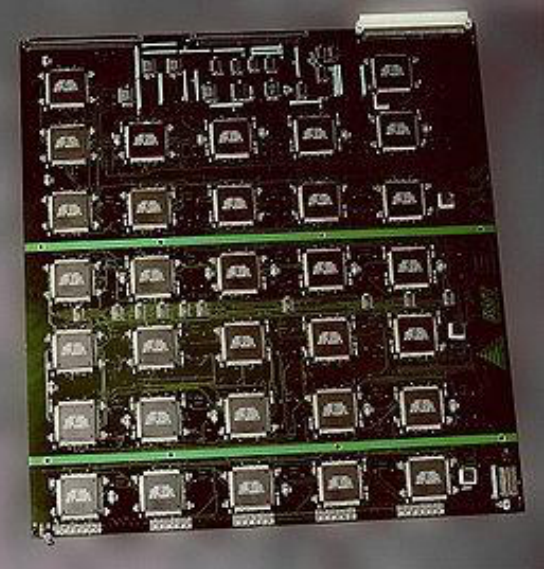
\includegraphics[width=60.06mm,height=156.52mm]{images/llm/page_042_img_01.png}%
\end{textblock*}

\newpage

% --- unit llm 43 ---
% === Halaman 43 (llm) ===

\begin{itemize}
  \item Their motivation was to show that DES was breakable in practice as well as in theory: "There are many people who will not believe a truth until they can see it with their own eyes. Showing them a physical machine that can crack DES in a few days is the only way to convince some people that they really cannot trust their security to DES."
  \item The machine brute-forced a key in a little more than 2 days search.
\end{itemize}

\newpage

% --- unit llm 44 ---
% === Halaman 44 (llm) ===

\begin{itemize}
  \item Pengisian kotak-S DES masih menjadi misteri. Nilai-nilai awal S-box sudah diubah.
  \item Sebenarnya delapan putaran sudah cukup untuk membuat cipherteks sebagai fungsi acak dari setiap bit plainteks dan setiap bit kunci.
  \item Namun dari penelitian dengan melakukan kriptanalisis, DES dengan jumlah putaran yang kurang dari 16 ternyata dapat dipecahkan dengan \textit{known-plaintext attack}.
\end{itemize}

\newpage

% --- unit llm 45 ---
% === Halaman 45 (llm) ===

\vspace{160.38mm}

Triple DES (3DES)

% deskripsi: Teks dekoratif besar berwarna biru yang bertuliskan '3DES Triple Data Encryption Standard'
% bbox normalisasi: [0.0900, 0.1900, 0.4000, 0.7300]
\begin{textblock*}{65.10mm}(18.90mm,56.43mm)
\noindent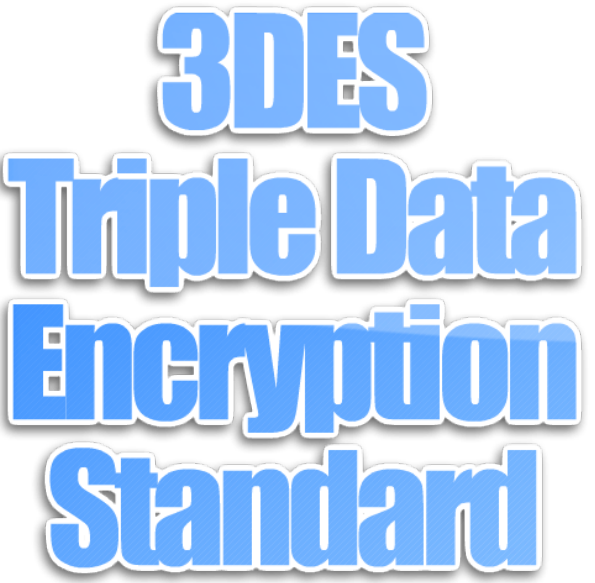
\includegraphics[width=65.10mm,height=160.38mm]{images/llm/page_045_img_01.png}%
\end{textblock*}

\newpage

% --- unit llm 46 ---
% === Halaman 46 (llm) ===

\section*{DES Berganda}

\begin{itemize}
    \item Karena DES mempunyai potensi kelemahan pada \textit{brute force attack}, maka dibuat varian dari DES.
    \item Varian DES yang paling luas digunakan adalah DES berganda (\textit{multiple DES}).
    \item DES berganda adalah enkripsi berkali-kali dengan DES dan menggunakan kunci ganda.
    \item Tinjau dua macam DES berganda:
    \begin{enumerate}
        \item \textit{Double DES}
        \item \textit{Triple DES (3DES)}
    \end{enumerate}
\end{itemize}

\newpage

% --- unit llm 47 ---
% === Halaman 47 (llm) ===

\section*{Double DES}

\vspace{89.10mm}

\begin{itemize}
    \item Menggunakan 2 buah kunci eksternal, $K_1$ dan $K_2$.
    \item Enkripsi: \[ C = E_{K_2}(E_{K_1}(P)) \]
    \item Dekripsi: \[ P = D_{K_1}(D_{K_2}(C)) \]
\end{itemize}

\vspace{30mm}

\vspace{30mm}

% deskripsi: Diagram alir proses enkripsi Double DES yang menunjukkan plaintext P melewati dua tahap enkripsi (E) menggunakan kunci K1 dan K2 untuk menghasilkan ciphertext C.
% bbox normalisasi: [0.3950, 0.2700, 0.8300, 0.5700]
\begin{textblock*}{91.35mm}(82.95mm,80.19mm)
\noindent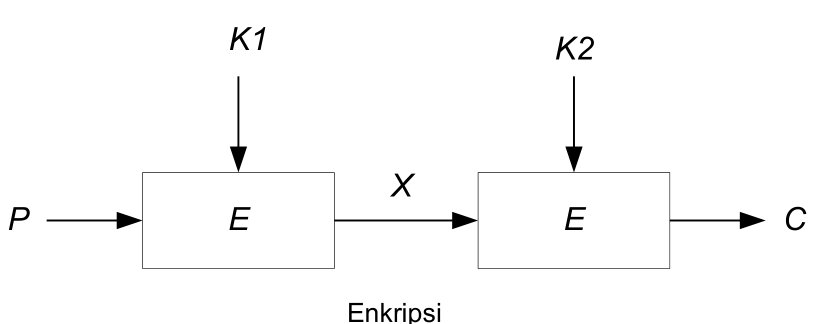
\includegraphics[width=91.35mm,height=89.10mm]{images/llm/page_047_img_01.png}%
\end{textblock*}

% deskripsi: Diagram alir proses dekripsi Double DES yang menunjukkan ciphertext C melewati dua tahap dekripsi (D) menggunakan kunci K2 dan K1 untuk menghasilkan plaintext P.
% bbox normalisasi: [0.3950, 0.6200, 0.8300, 0.9000]
\begin{textblock*}{91.35mm}(82.95mm,184.14mm)
\noindent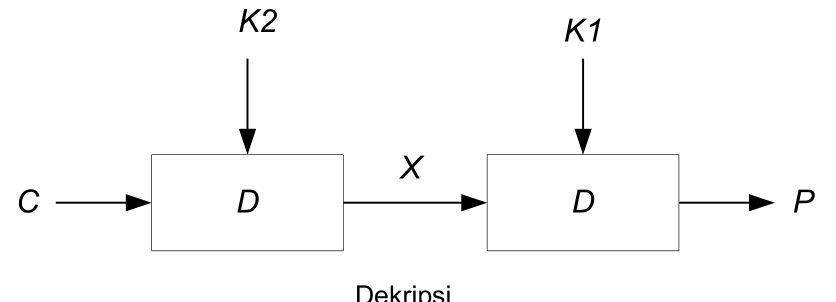
\includegraphics[width=91.35mm,height=83.16mm]{images/llm/page_047_img_02.png}%
\end{textblock*}

\newpage

% --- unit llm 48 ---
% === Halaman 48 (llm) ===

\vspace{238.79mm}

\begin{itemize}
    \item Kelemahan \textit{Double DES}: serangan \textit{meet-in-the-middle attack}:
    \item Dari pengamatan,
    \[ C = E_{K2}(E_{K1}(P)) \]
    maka
    \[ X = E_{K1}(P) = D_{K2}(C) \]
\end{itemize}

\vspace{40mm}

\begin{itemize}
    \item Misalkan kriptanalisis memiliki potongan $C$ dan $P$ yang berkorepsonden (\textit{known-plaintext attack}).
    \item Enkripsi $P$ untuk semua kemungkinan nilai $K1$ (yaitu sebanyak $2^{56}$ kemungkinan kunci). Hasilnya adalah semua nilai $X$
    \item Simpan semua nilai $X$ ini di dalam tabel
\end{itemize}

% deskripsi: Diagram proses enkripsi dan dekripsi Double DES yang menunjukkan serangan meet-in-the-middle, dengan aliran P ke C melalui enkripsi dua tahap (K1, K2) dan aliran C ke P melalui dekripsi dua tahap (K2, K1), bertemu di nilai perantara X.
% bbox normalisasi: [0.0600, 0.1080, 0.9400, 0.9120]
\begin{textblock*}{184.80mm}(12.60mm,32.08mm)
\noindent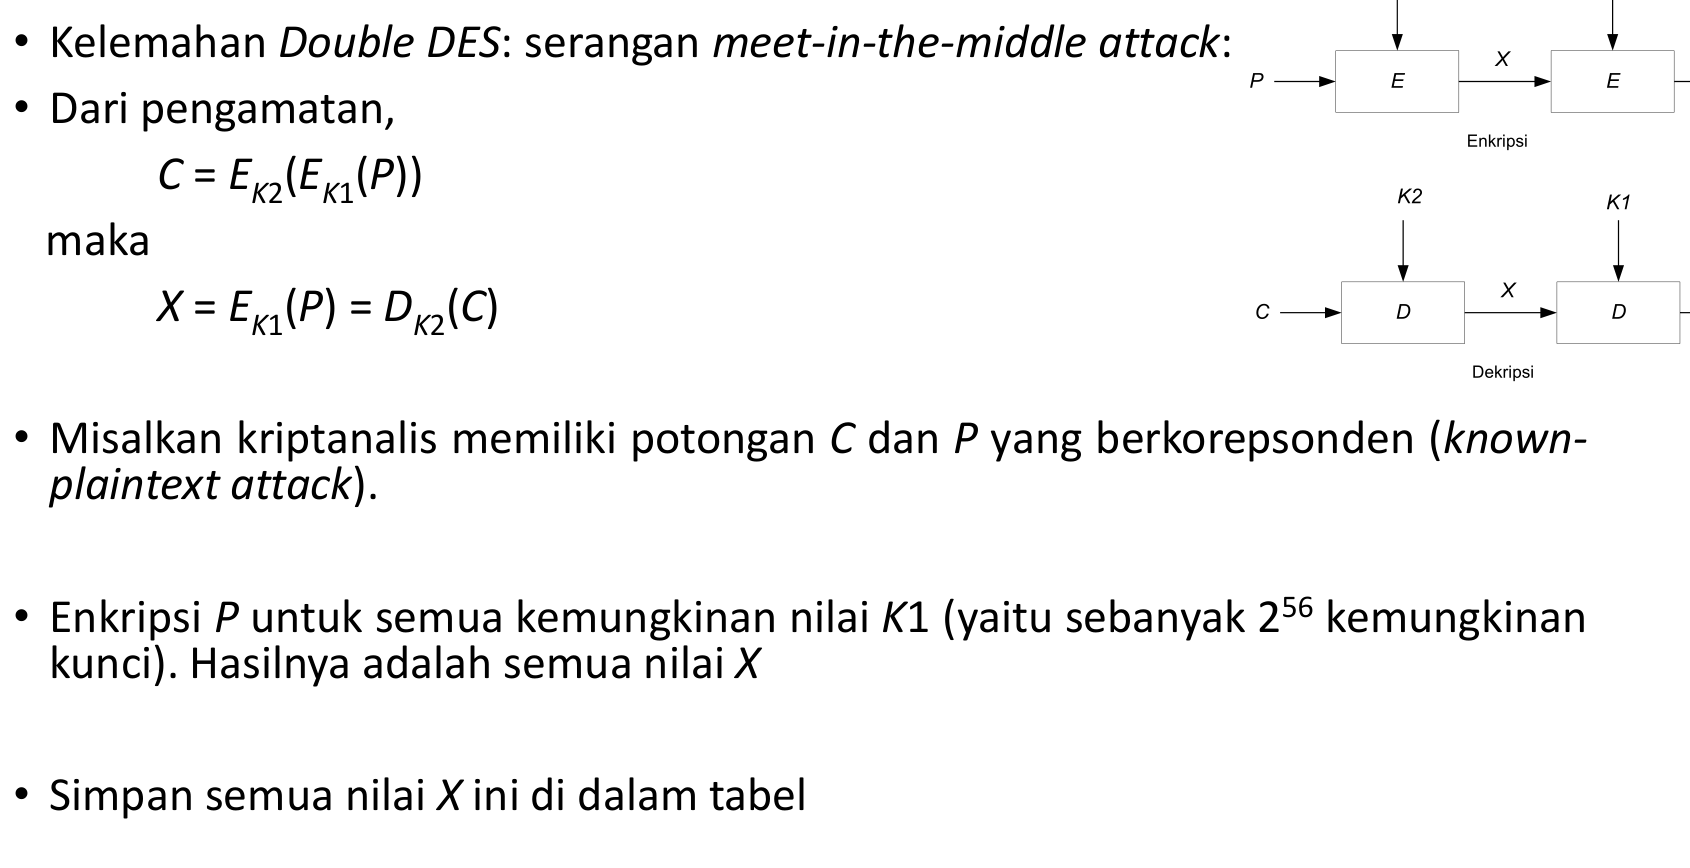
\includegraphics[width=184.80mm,height=238.79mm]{images/llm/page_048_img_01.png}%
\end{textblock*}

% bbox perkiraan otomatis: Diagram proses enkripsi dan dekripsi Double DES yang menunjukkan serangan meet-in-the-middle, dengan aliran P ke C melalui enkripsi dua tahap (K1, K2) dan aliran C ke P melalui dekripsi dua tahap (K2, K1), bertemu di nilai perantara X.

\newpage

% --- unit llm 49 ---
% === Halaman 49 (llm) ===

\vspace{118.80mm}

\begin{itemize}
    \item Berikutnya, dekripsi $C$ dengan semua semua kemungkinan nilai $K2$ (yaitu sebanyak $2^{56}$ kemungkinan kunci).
    \item Bandingkan semua hasil dekripsi ini dengan elemen di dalam tabel tadi. Jika ada yang sama, maka dua buah kunci, $K1$ dan $K2$, telah ditemukan.
    \item Tes kedua kunci ini dengan pasangan plainteks-cipherteks lain yang diketahui. Jika kedua kunci tersebut menghasilkan cipherteks atau plainteks yang benar, maka $K1$ dan $K2$ tersebut merupakan kunci yang benar
\end{itemize}

% deskripsi: Tabel perbandingan hasil enkripsi dan dekripsi untuk menemukan kunci K1 dan K2, menampilkan kolom K1, X, K2, dan X dengan beberapa nilai biner yang ditandai warna merah untuk menunjukkan kecocokan.
% bbox normalisasi: [0.5900, 0.4000, 0.9600, 0.8000]
\begin{textblock*}{77.70mm}(123.90mm,118.80mm)
\noindent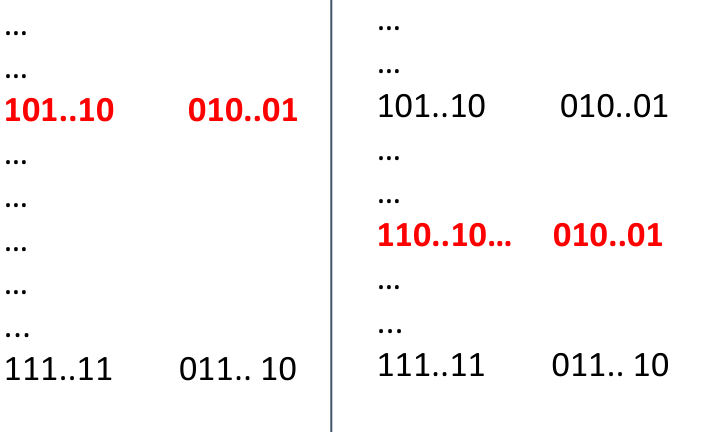
\includegraphics[width=77.70mm,height=118.80mm]{images/llm/page_049_img_01.png}%
\end{textblock*}

\newpage

% --- unit llm 50 ---
% === Halaman 50 (llm) ===

\section*{Triple DES (TDES)}

\vspace{71.28mm}

\begin{itemize}
    \item Menggunakan DES tiga kali
    \item Bertujuan untuk mencegah \textit{meet-in-the-middle attack}.
    \item Bentuk umum Triple DES (mode EEE):
    \begin{align*}
        \text{Enkripsi: } C &= E_{K3}(E_{K2}(E_{K1}(P)))\\ 
        \text{Dekripsi: } P &= D_{K1}(D_{K2}(D_{K3}(C)))
    \end{align*}
\end{itemize}

\vspace{20mm}

% deskripsi: Diagram blok proses enkripsi Triple DES (EEE) dengan tiga tahap enkripsi (E) menggunakan kunci K1, K2, dan K3 secara berurutan.
% bbox normalisasi: [0.5120, 0.3970, 0.9900, 0.6370]
\begin{textblock*}{100.38mm}(107.52mm,117.91mm)
\noindent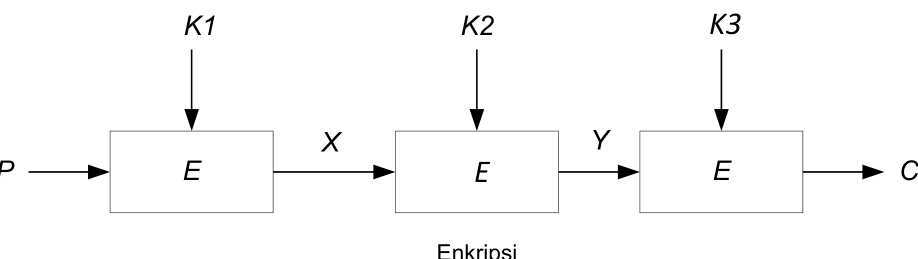
\includegraphics[width=100.38mm,height=71.28mm]{images/llm/page_050_img_01.png}%
\end{textblock*}

% deskripsi: Diagram blok proses dekripsi Triple DES (EEE) dengan tiga tahap dekripsi (D) menggunakan kunci K3, K2, dan K1 secara berurutan.
% bbox normalisasi: [0.5120, 0.6950, 0.9900, 0.9350]
\begin{textblock*}{100.38mm}(107.52mm,206.41mm)
\noindent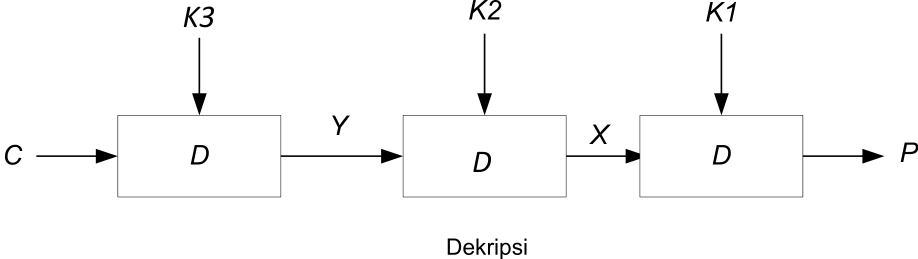
\includegraphics[width=100.38mm,height=71.28mm]{images/llm/page_050_img_02.png}%
\end{textblock*}

\newpage

% --- unit llm 51 ---
% === Halaman 51 (llm) ===

\begin{itemize}
    \item Untuk menyederhanakan TDES, maka langkah di tengah diganti dengan D (mode EDE).
    \item Ada dua versi TDES dengan mode EDE:
    \begin{itemize}
        \item Menggunakan 2 kunci
        \item Menggunaakn 3 kunci
    \end{itemize}
    \item Kenapa EDE? Supaya kompatibel dengan single DES:
\end{itemize}

\newpage

% --- unit llm 52 ---
% === Halaman 52 (llm) ===

\section*{Triple DES}

\vspace{71.28mm}

\textbf{Triple DES dengan 2 kunci (56 + 56 = 112 bit)}

\vspace{20mm}

\vspace{20mm}

% deskripsi: Diagram proses enkripsi Triple DES dengan 2 kunci (K1, K2, K1) yang terdiri dari tahap enkripsi (E), dekripsi (D), dan enkripsi (E) kembali.
% bbox normalisasi: [0.1800, 0.3400, 0.6700, 0.5800]
\begin{textblock*}{102.90mm}(37.80mm,100.98mm)
\noindent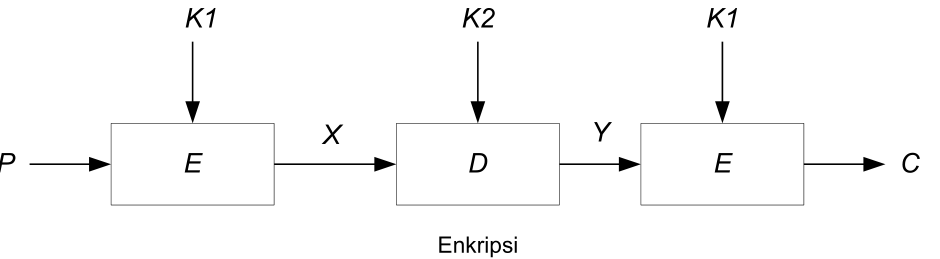
\includegraphics[width=102.90mm,height=71.28mm]{images/llm/page_052_img_01.png}%
\end{textblock*}

% deskripsi: Diagram proses dekripsi Triple DES dengan 2 kunci yang merupakan kebalikan dari proses enkripsi, terdiri dari tahap dekripsi (D), enkripsi (E), dan dekripsi (D) kembali.
% bbox normalisasi: [0.1800, 0.6200, 0.6700, 0.8700]
\begin{textblock*}{102.90mm}(37.80mm,184.14mm)
\noindent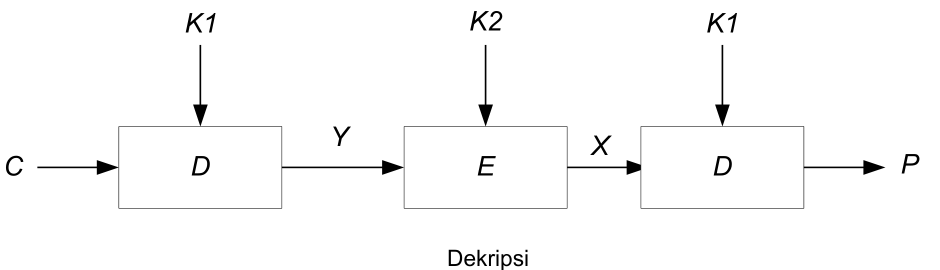
\includegraphics[width=102.90mm,height=74.25mm]{images/llm/page_052_img_02.png}%
\end{textblock*}

\newpage

% --- unit llm 53 ---
% === Halaman 53 (llm) ===

\vspace{109.89mm}

\textbf{Triple DES dengan 3 kunci} $(56 + 56 + 56 = 168)$

% deskripsi: Diagram alur proses Enkripsi dan Dekripsi Triple DES dengan 3 kunci berbeda (K1, K2, K3) yang menunjukkan urutan operasi Encrypt (E) dan Decrypt (D).
% bbox normalisasi: [0.0600, 0.1080, 0.9400, 0.9120]
\begin{textblock*}{184.80mm}(12.60mm,32.08mm)
\noindent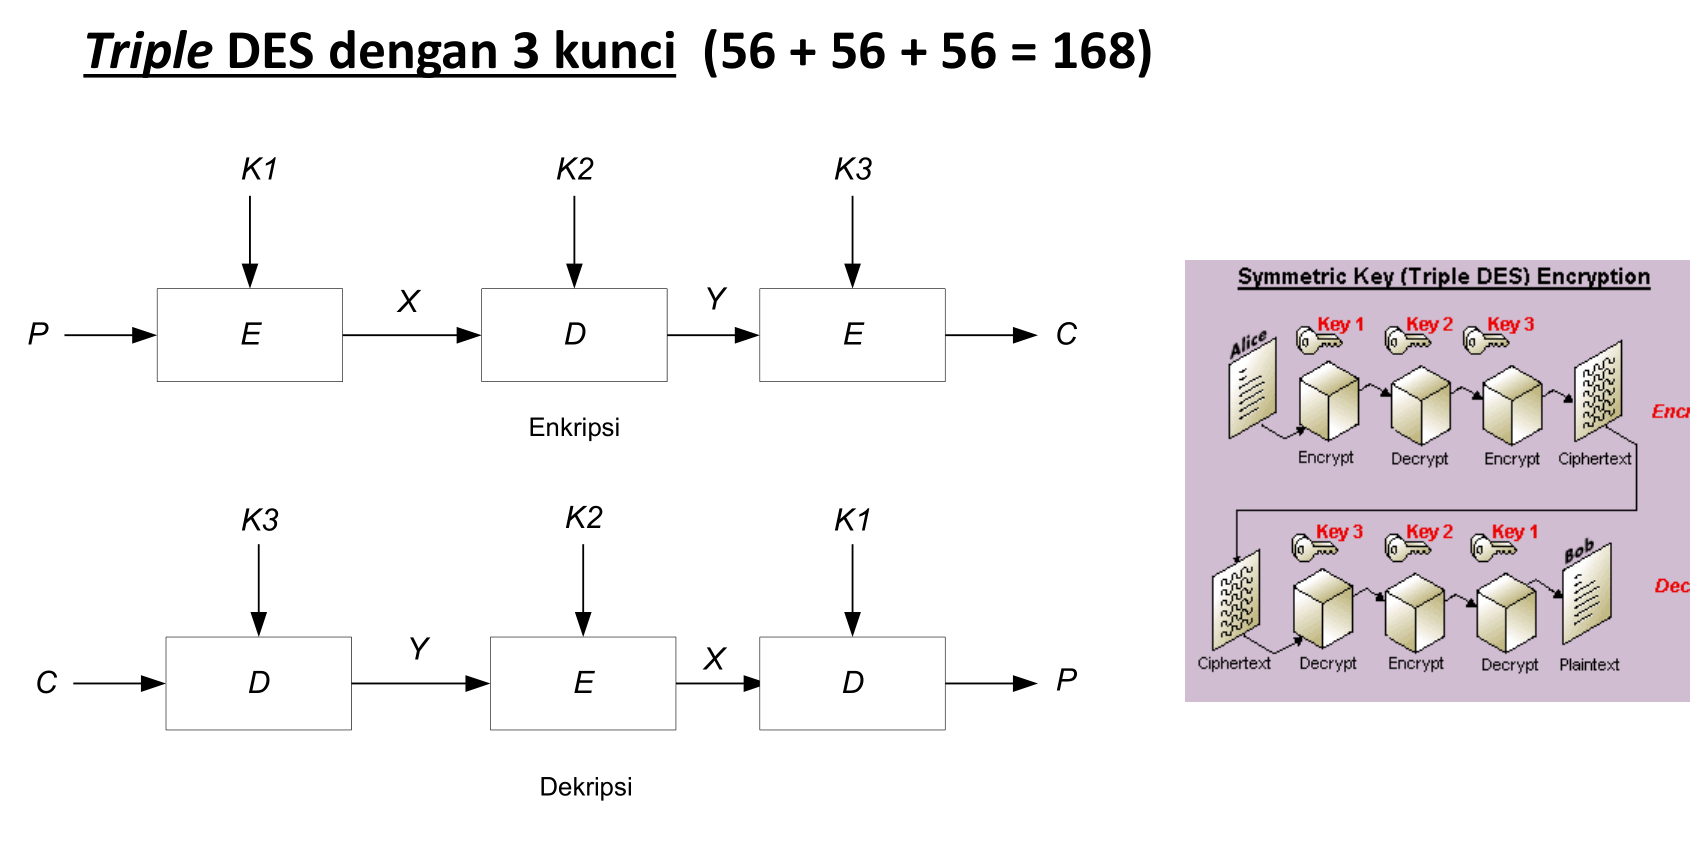
\includegraphics[width=184.80mm,height=238.79mm]{images/llm/page_053_img_01.png}%
\end{textblock*}

% deskripsi: Ilustrasi visual enkripsi dan dekripsi simetrik Triple DES yang melibatkan Alice dan Bob, menampilkan penggunaan tiga kunci berbeda dan proses pengubahan Plaintext menjadi Ciphertext dan sebaliknya.
% bbox normalisasi: [0.6800, 0.3100, 0.9800, 0.6800]
\begin{textblock*}{63.00mm}(142.80mm,92.07mm)
\noindent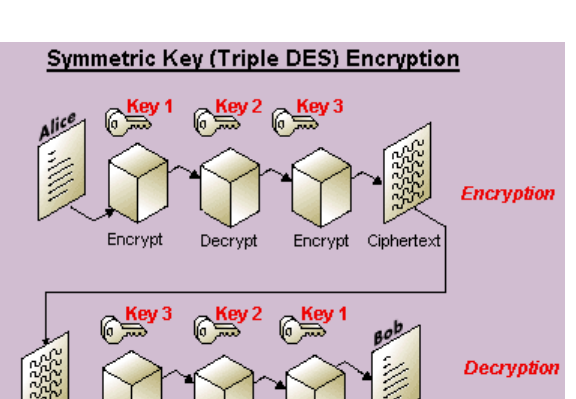
\includegraphics[width=63.00mm,height=109.89mm]{images/llm/page_053_img_02.png}%
\end{textblock*}

% bbox perkiraan otomatis: Diagram alur proses Enkripsi dan Dekripsi Triple DES dengan 3 kunci berbeda (K1, K2, K3) yang menunjukkan urutan operasi Encrypt (E) dan Decrypt (D).

\end{document}
